\documentclass[9pt, xcolor=table]{beamer}
\usetheme{Warsaw}

\usepackage[utf8]{inputenc}
\usepackage[italian]{babel}
\usepackage{graphicx}
\usepackage{listings}
\usepackage[ruled, vlined]{algorithm2e}

\definecolor{cadmiumgreen}{rgb}{0.0, 0.42, 0.24}

\lstset{language=R,
	basicstyle=\tiny\ttfamily,
	stringstyle=\color{cadmiumgreen},
	otherkeywords={0,1,2,3,4,5,6,7,8,9},
	morekeywords={TRUE,FALSE},
	deletekeywords={data,frame,length,as,character},
	keywordstyle=\color{blue},
	commentstyle=\color{cadmiumgreen},
	frame=single,
	breaklines=true,
	showstringspaces=false
}

\graphicspath{ {./imgs/} }

\title{Predire la Sopravvivenza sul Titanic con gli Alberi Decisionali}

\author[Elia Mercatanti]{Elia Mercatanti}

\institute[UNIFI]
{
	Università degli Studi di Firenze\\
	Scuola di Scienze Matematiche, Fisiche e Naturali\\
	Corso di Laurea Magistrale in Informatica - Data Science
}

\date[Contest MASL]
{Contest MASL, Dicembre 2020}

\begin{document}
	\begin{frame}
		\maketitle
	\end{frame}

	\begin{frame}{L'Affondamento del Titanic}
		\centering
		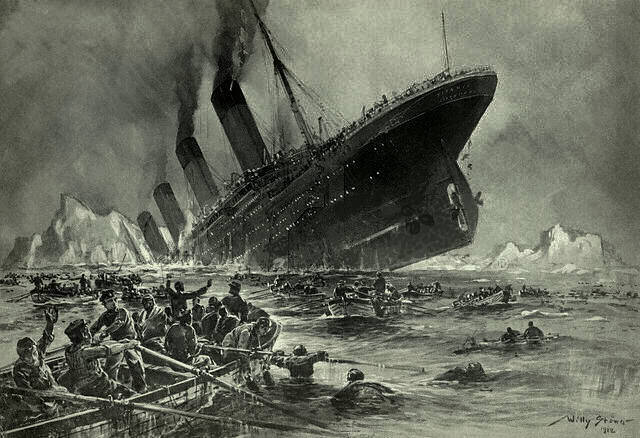
\includegraphics[scale=0.33]{titanic}
		
		\vfill
		
		\begin{itemize}
			\item Il 15 aprile 1912, durante il suo viaggio inaugurale, considerato
			"inaffondabile", affondò dopo essersi scontrato con un iceberg.
			\item Scarse scialuppe di salvataggio, provocando la morte di 1502
			su 2224 passeggeri e membri dell'equipaggio.
			\item Sembra che alcuni gruppi di persone fossero più propensi a
			sopravvivere rispetto ad altri.
		\end{itemize}
	\end{frame}

	\begin{frame}{Scopo del Progetto}
		\begin{block}{Scopo del Progetto}
			\begin{itemize}
				\item Rispondere alla domanda: "Che tipo di persone avevano
				maggiori probabilità di sopravvivere?".
				\item Predire quali passeggeri del Titanic sono sopravvissuti o meno.
				\item Uso degli alberi di decisione in R. Utilizzando diversi pacchetti e confrontando i risultati ottenuti.
			\end{itemize}
		\end{block}
    \end{frame}

	\begin{frame}{Presentazione del Dataset del Titanic}
		\begin{block}{Dataset}
			I dati sono stati suddivisi in due gruppi:
			\begin{itemize}
				\item Set di \textbf{training} (\textit{titanic-train.csv}). Contiene la variabile
				"\textit{Survived}", variabile di risposta. Per addestrare e valutare i
				modelli, diviso appositamente.
				\item Set di \textbf{test} (\textit{titanic-test.csv}). Mancante della variabile
				"\textit{Survived}". Per analisi del dataset.
				\item \textbf{Osservazioni}: 891 (train set) + 418 (test set).
				\item \textbf{Variabili}: 12 in totale che descrivono alcune caratteristiche
				dei passeggeri del Titanic.
			\end{itemize}
		\end{block}
	
		\begin{table}[]
			\resizebox{\textwidth}{!}{
			\begin{tabular}{c|c|c|c|c|c|c|c|c|c|c|c}
				\hline
				\textbf{PassengerId} & \textbf{Survived} & \textbf{Pclass} & \textbf{Name}                                                & \textbf{Sex}    & \textbf{Age} & \textbf{SibSp} & \textbf{Parch} & \textbf{Ticket}   & \textbf{Fare}    & \textbf{Cabin} & \textbf{Embarked} \\ \hline
				1 & 0 & 3 & Braund, Mr. Owen Harris  & male   & 22 & 1 & 0 & A/5 21171        & 7.25  &  & S \\
				2           & 1        & 1      & Cumings, Mrs. John Bradley (Florence Briggs Thayer) & female & 38  & 1     & 0     & PC 17599 & 71.2833 & C85   & C        \\
				3 & 1 & 3 & Heikkinen, Miss. Laina   & female & 26 & 0 & 0 & STON/O2. 3101282 & 7.925 &  & S \\
				4           & 1        & 1      & Futrelle, Mrs. Jacques Heath (Lily May Peel)        & female & 35  & 1     & 0     & 113803   & 53.1    & C123  & S        \\
				5 & 0 & 3 & Allen, Mr. William Henry & male   & 35 & 0 & 0 & 373450           & 8.05  &  & S \\ \hline
			\end{tabular}
		}
		\end{table}
	\end{frame}

	\begin{frame}{Presentazione del Dataset del Titanic}
		\begin{itemize}
			\item \textbf{Survival}: indica se il passeggero è sopravvissuto o meno (0 = No, 1 = Si). Rappresenta la nostra variabile di risposta.
			\item \textbf{PassengerId}: id assegnato al passeggero.
			\item \textbf{Name}: nome, cognome e titolo del passeggero.
			\item \textbf{Pclass}: classe del biglietto (1 = 1st, 2 = 2nd, 3 = 3rd).
			\item \textbf{Sex}: sesso del passeggero.
			\item \textbf{Age}: età in anni del passeggero.
			\item \textbf{Sibsp}: numero di fratelli/coniugi a bordo del Titanic.
			\item \textbf{Parch}: numero di genitori/figli a bordo del Titanic.
			\item \textbf{Ticket}: numero del biglietto.
			\item \textbf{Fare}: tariffa del passeggero.
			\item \textbf{Cabin}: numero della cabina.
			\item \textbf{Embarked}: porto di imbarcazione (C = Cherbourg, Q =
			Queenstown, S = Southampton).
		\end{itemize}
	\end{frame}

	\begin{frame}{Gestione Dati Mancanti}
			\begin{columns}
			\column{0.5\textwidth}
			\centering
			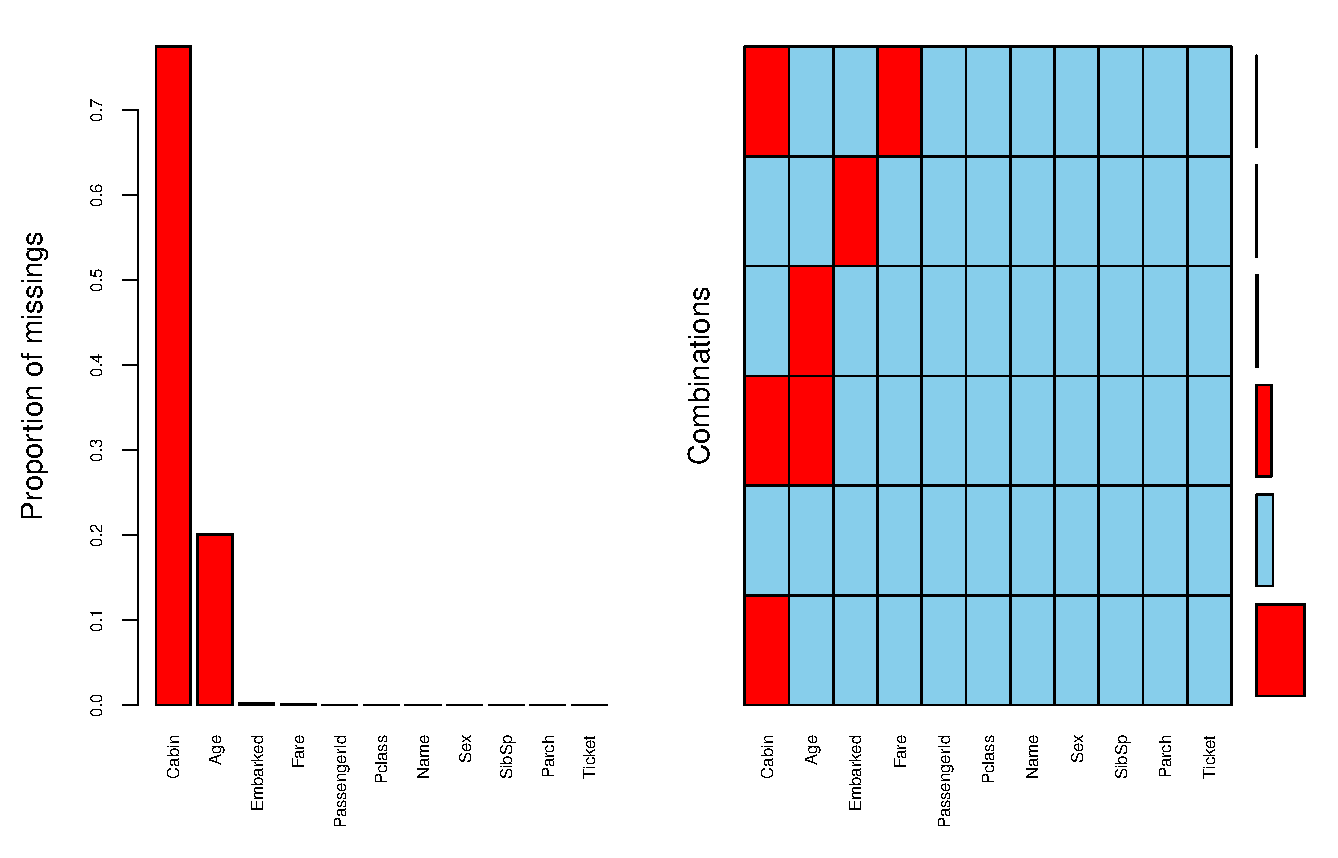
\includegraphics[scale=0.26]{missing-data-prop}
			\column{0.5\textwidth}
			\centering
			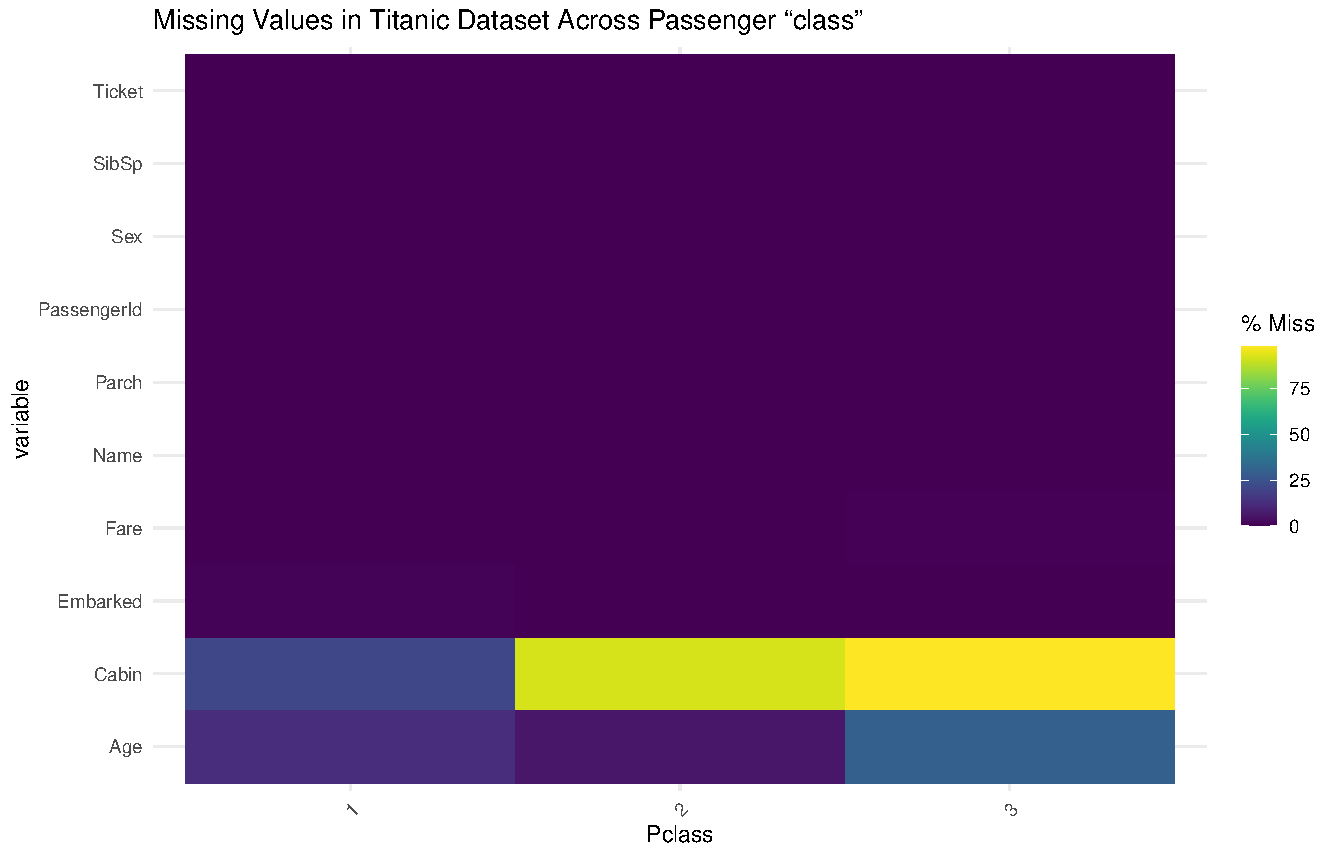
\includegraphics[scale=0.26]{missing-data-pclass}
		\end{columns}		
	\end{frame}

	\begin{frame}{Gestione Dati Mancanti}
		\begin{itemize}
			\item Uniamo i dati di train e test per analizzare meglio il dataset.
			\item \textbf{Cabin}: troppi valori mancanti, rischia di alterare un modello.
			Viene dunque rimossa.
			\item \textbf{Age}: probabilmente uno dei fattori più importanti. Sfruttiamo l'età mediane tra Sex e Pclass per stimarne i valori mancanti.
			
			\lstinputlisting[firstline=73, lastline=79]{../titanic-decision-trees.R}
			
			\item \textbf{Embarked}: ha due soli valori mancanti. Li riempiamo
			semplicemente con il porto più comune (Southampton, S).
			\item \textbf{Fare}: l'unico valore mancante possiamo sostituirlo con la
			mediana.
		\end{itemize}
	\end{frame}

	\begin{frame}{Esplorazione e Visualizzazione dei Dati}
		\begin{columns}
			\column{0.5\textwidth}
			\centering
			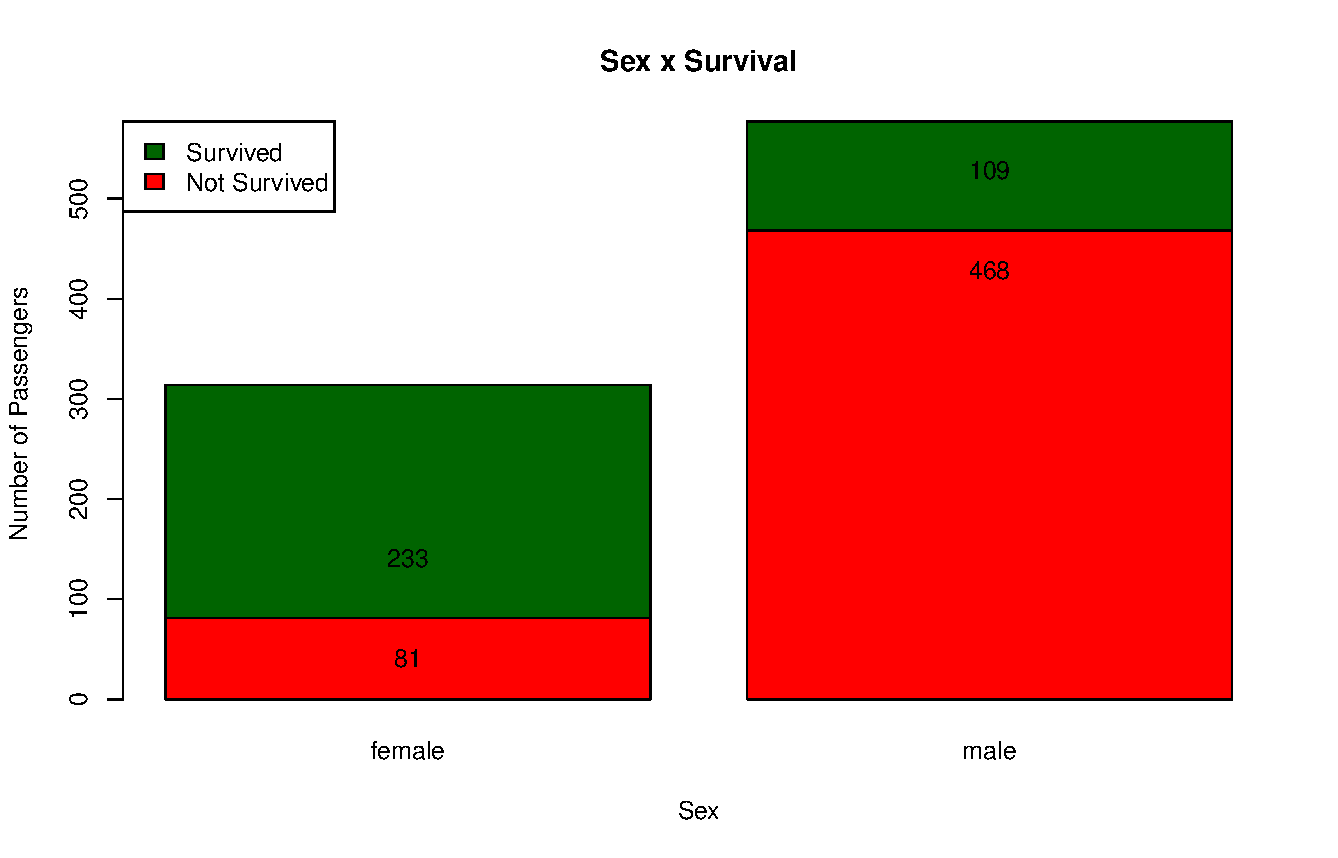
\includegraphics[scale=0.26]{barplot-sex-survival}
			\column{0.5\textwidth}
			\centering
			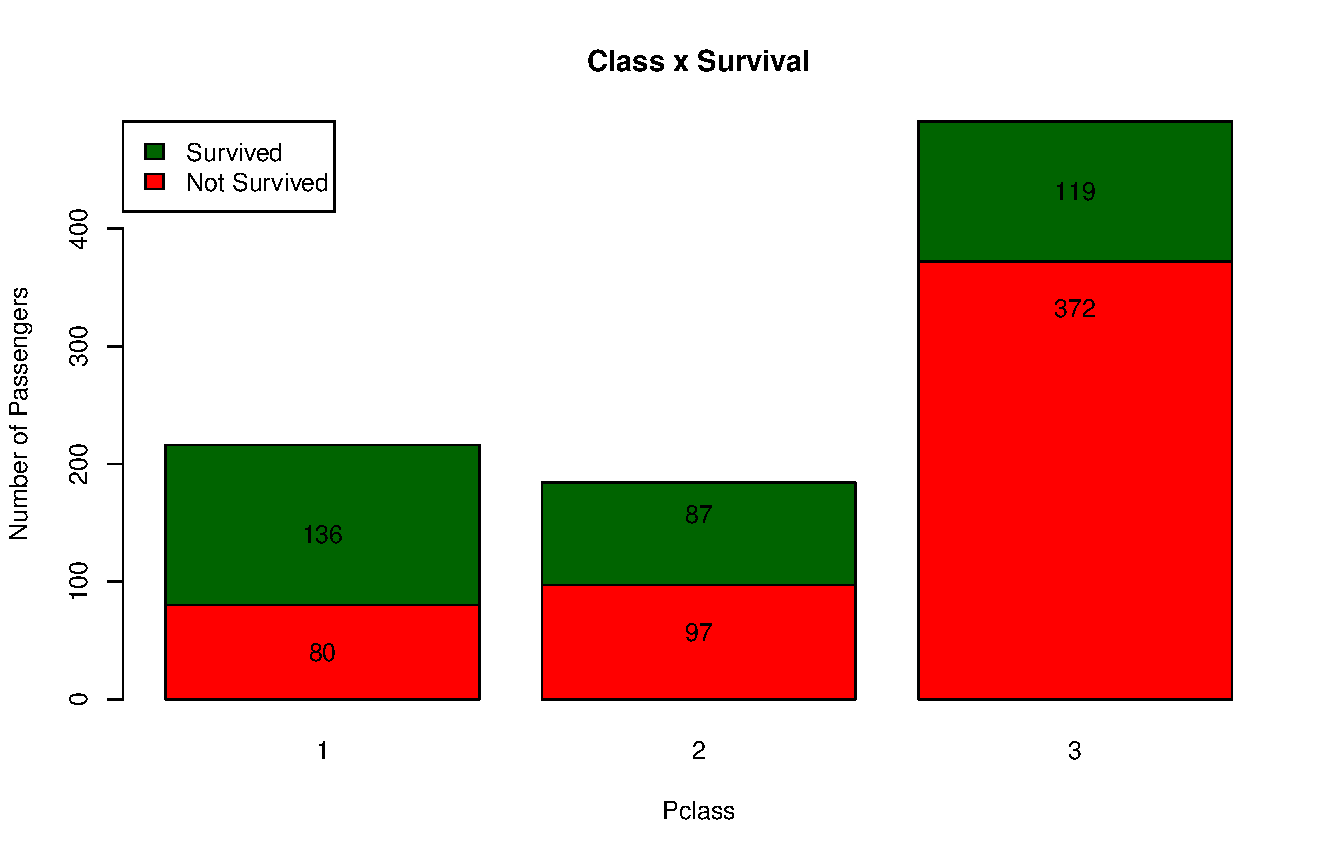
\includegraphics[scale=0.26]{barplot-class-survival}
		\end{columns}
		\begin{columns}
			\column{0.5\textwidth}
			\centering
			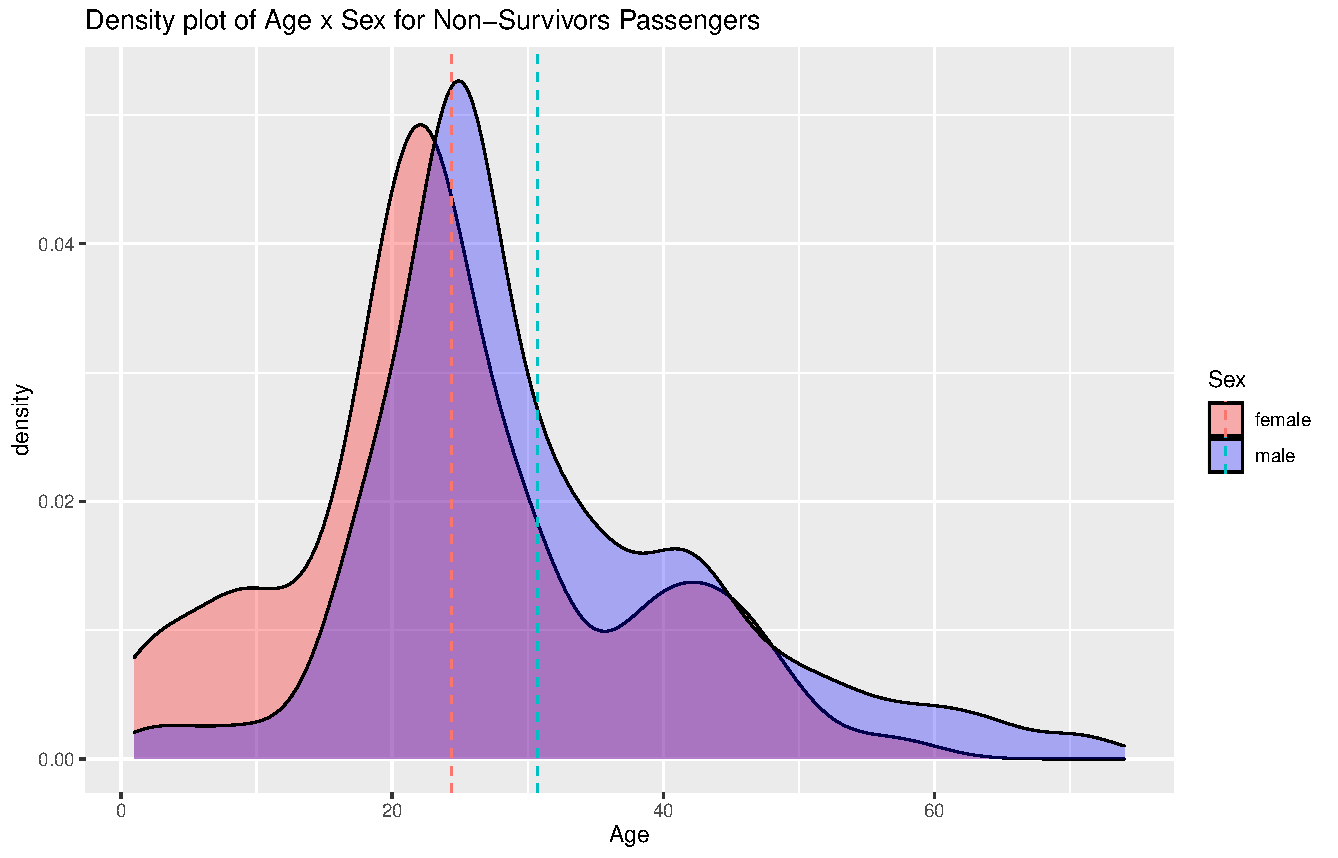
\includegraphics[scale=0.26]{density-age-sex-notsurvived}
			\column{0.5\textwidth}
			\centering
			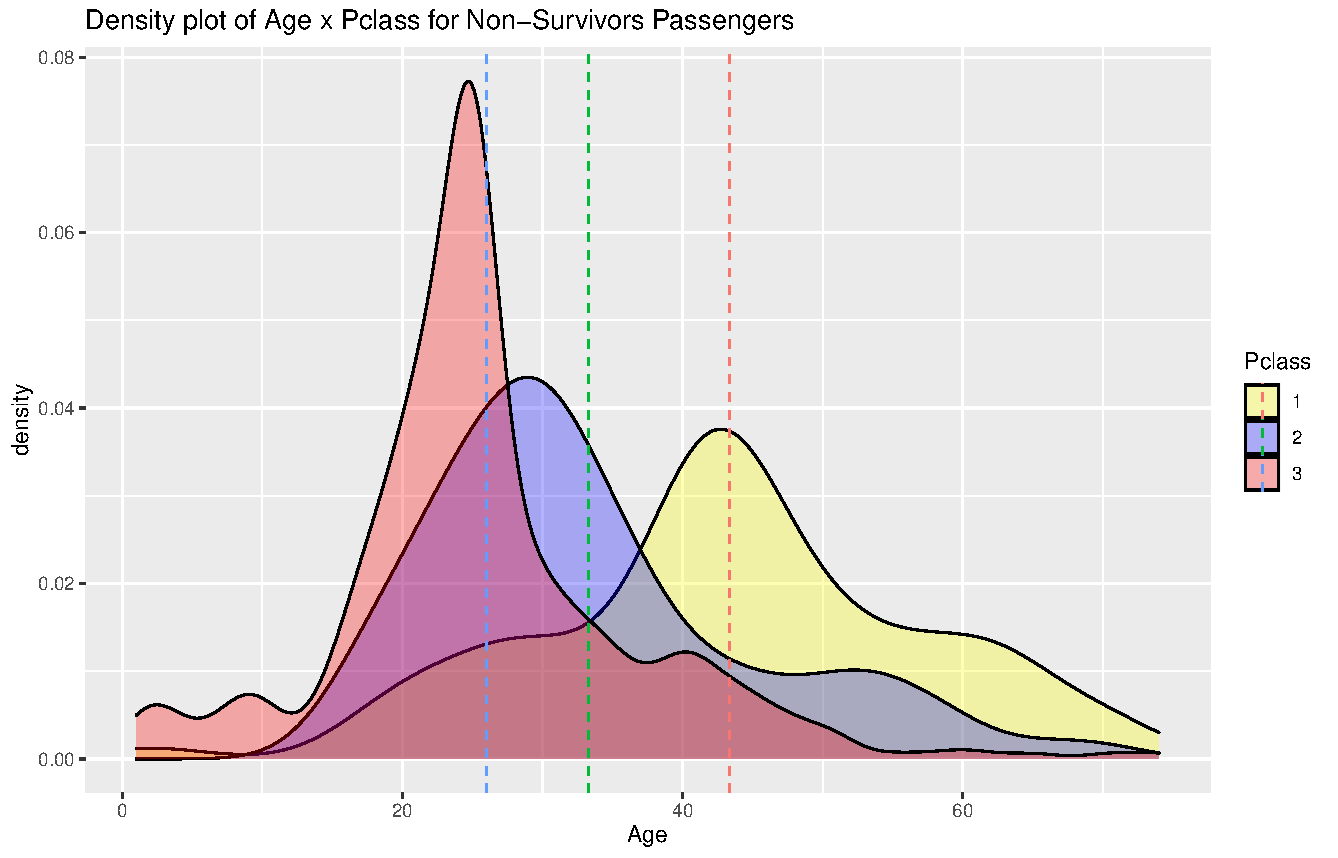
\includegraphics[scale=0.26]{density-age-pclass-notsurvived}
		\end{columns}
	\end{frame}

	\begin{frame}{Feature Extraction - Titolo}
		\begin{itemize}
			\item \textbf{Title}: Utilizzato per capire il grado nella società, utile nella classificazione. Trasmette gli effetti interattivi tra Age e Sex.
			\begin{itemize}
				\item Possiamo raggruppare i titoli in "MR", "MISS", "MRS",
				"MASTER" e "Other" per i più rari.
			\end{itemize}
		\end{itemize}
	
		\centering
		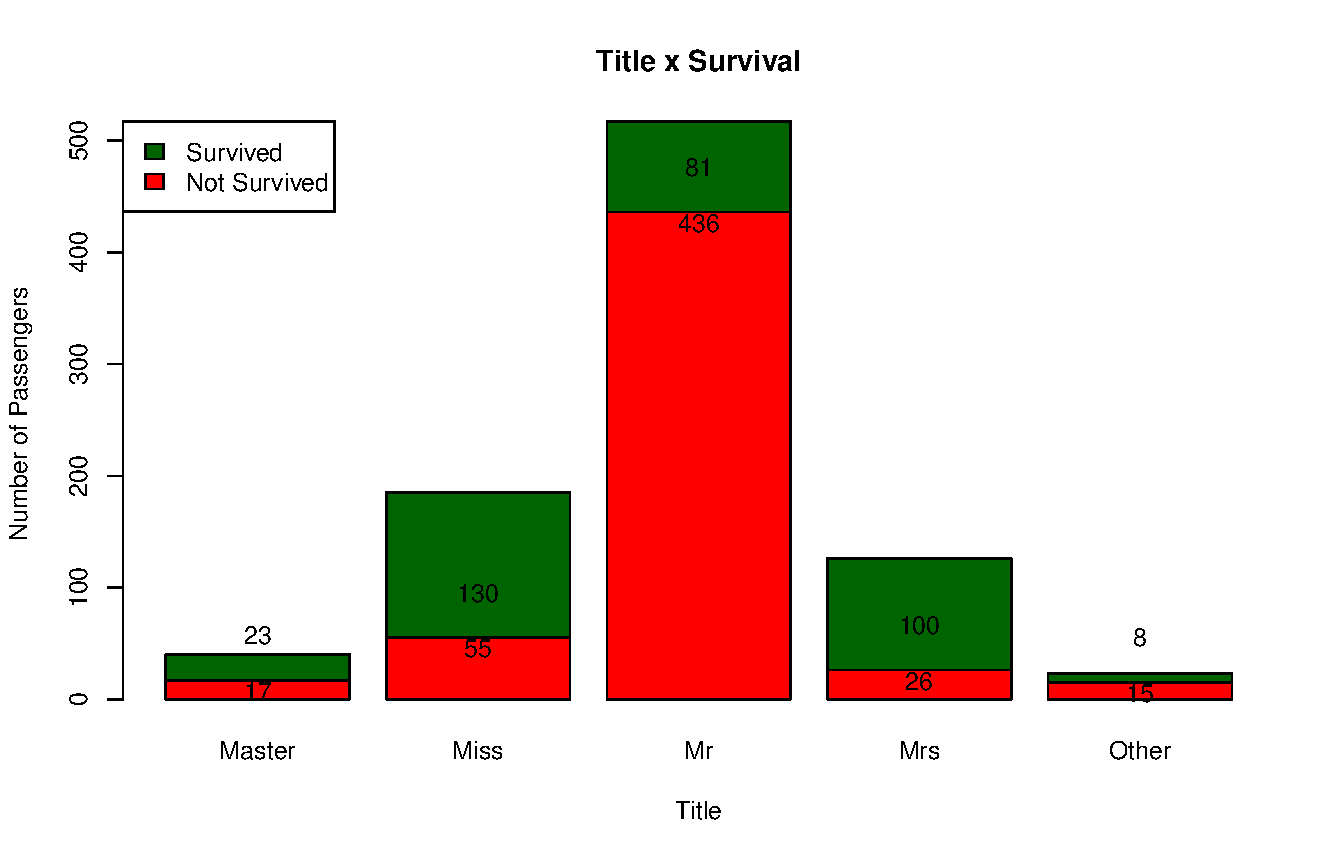
\includegraphics[scale=0.4]{barplot-title-survival}
	\end{frame}

	\begin{frame}{Feature Extraction - Family Size e IsAlone}
		\begin{itemize}
			\item \textbf{FamilySize}: la dimensione della famiglia imbarcata potrebbe
			essere un fattore interessante (\textbf{SibSp} + \textbf{Parch} + 1).
			
			\centering
			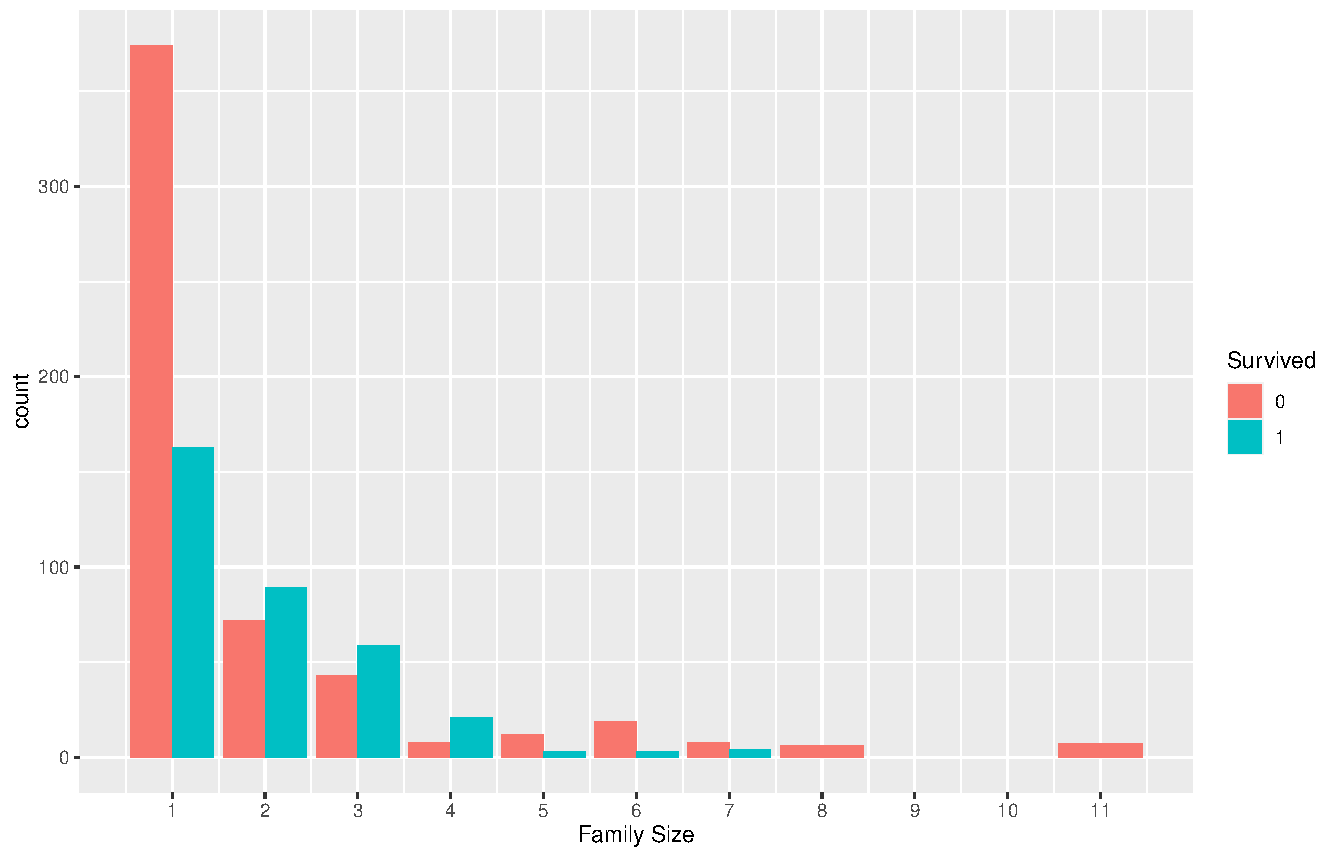
\includegraphics[scale=0.38]{barplot-familysize}
			
			\item \textbf{IsAlone}: possiamo vedere che le persone single hanno un più alto tasso di "morte" rispetto alle altre persone.
		\end{itemize}
	\end{frame}

	\begin{frame}{Feature Extraction - Fare e Dataset Finale}
		\begin{itemize}
			\item \textbf{Fare}: per rendere le tariffe più facili da analizzare, ed essendo continua, le raccogliamo in 4 gruppi di dimensioni omogenee (1 - \textbf{[0,7.9]}, 2 - \textbf{(7.9,14.5]}, 3 - \textbf{(14.5,31.3]}, 4 - \textbf{(31.3,512]}).
			
			\item Infine eliminiamo le variabili che non ci servono più e non contengono più informazioni rilevanti (\textit{PassengerId}, \textit{Name}, \textit{SibSp}, \textit{Parch}, \textit{Ticket}).
		\end{itemize}
	
		\vfill
	
		Di seguito viene mostrato il dataset finale che utilizzeremo.
		
		\begin{table}[]
			\resizebox{\textwidth}{!}{
			\begin{tabular}{c|c|c|c|c|c|c|c|c}
				\hline
				\textbf{Survived} & \textbf{Pclass} & \textbf{Sex}    & \textbf{Age} & \textbf{Fare} & \textbf{Embarked} & \textbf{Title} & \textbf{FamilySize} & \textbf{IsAlone} \\ \hline
				0        & 3      & male   & 22  & 1    & S        & Mr    & 2          & 0       \\
				1        & 1      & female & 38  & 4    & C        & Mrs   & 2          & 0       \\
				1        & 3      & female & 26  & 2    & S        & Miss  & 1          & 1       \\
				1        & 1      & female & 35  & 4    & S        & Mrs   & 2          & 0       \\
				0        & 3      & male   & 35  & 2    & S        & Mr    & 1          & 1       \\ \hline
			\end{tabular}
		}
		\end{table}
	\end{frame}

    \begin{frame}{Alberi Decisionali}
    	\begin{itemize}
    		\item Utilizzano un albero per passare dalle osservazioni su un elemento (\textbf{rami}) alle conclusioni sulla variabile obiettivo dell'elemento (\textbf{foglie}).
    		
    		\item \textbf{Classificazione}: le foglie rappresentano etichette di classe, i rami le congiunzioni di caratteristiche che portano a classi.
    	\end{itemize}
    
    	\vfill
    	
    	In questo progetto utilizzeremo quattro tipologie di alberi di decisione:
    	\begin{itemize}
    		\item \textbf{Classification And Regression Tree} (\textbf{CART}): partizionamento ricorsivo dello spazio dei predittori, nel quale ad ogni elemento viene assegnata una
    		classe di predizione.
    		
    		\item \textbf{Conditional Inference Trees}: approccio statistico che utilizza test non parametrici come criteri di split.
    		\item \textbf{Evolutionary Learning of Globally Optimal Trees} (\textbf{evtree}).
    		
    		\item \textbf{Bootstrap Aggregated} (\textbf{Bagged}): costruiscono più alberi decisionali ricampionando ripetutamente i dati di training con reimmissione e le previsioni sono effettuate con voto di maggioranza o con media dei risultati su tutti gli alberi.
    	\end{itemize}
    \end{frame}

	\begin{frame}{Alberi Decisionali - Vantaggi e Limitazioni}
		\textbf{Vantaggi}:
		\begin{itemize}
			\item Semplici da capire e interpretare.
			\item Sono in grado di gestire dati sia numerici che categorici.
			\item Richiedono poca preparazione dei dati.
			\item Funzionano bene con set di dati di grandi dimensioni.
			\item Rispecchiano il processo decisionale umano più da vicino.
			\item Robusti contro la collinearità.
			\item La gerarchia degli attributi riflette l'importanza di essi.
		\end{itemize}
	
		\vfill
		
		\textbf{Limitazioni}:
		\begin{itemize}
			\item Gli alberi possono essere poco robusti.
			\item L'apprendimento di un albero ottimale è NP-completo.
			\item Gli albero decisionali possono andare in \textit{Overfitting}.
		\end{itemize}
	\end{frame}

	\begin{frame}{Alberi Decisionali - CART per Classificazione}
		\begin{block}{Obiettivo}
			Ottenere una segmentazione gerarchica di un insieme di unità statistiche mediante l’individuazione di “regole” che sfruttano la relazione esistente tra classe e predittori.
		\end{block}
		
		\vfill
		
		\begin{itemize}
			\item Le regole basate sui valori delle variabili vengono selezionate per ottenere il migliore \textbf{split} per differenziare le osservazioni in base alla variabile dipendente.
			
			\item Una regola divide un nodo in due \textbf{nodi figli}, lo stesso processo viene applicato a ciascun nodo "figlio" (ricorsivamente).
			
			\item Lo splitting si interrompe quando non è possibile ottenere più un guadagno (Gain) o viene soddisfatto un criterio di arresto.
		\end{itemize}
	
		\vfill
	
		Ogni osservazione rientra in un unico \textbf{nodo terminale} definito in modo univoco da un insieme di regole.
	\end{frame}

	\begin{frame}{Alberi Decisionali - CART per Classificazione}
		\begin{block}{Valutazione degli Split}
			\begin{itemize}
				\item Favorire l'\textbf{omogeneità} interna dei nodi ed \textbf{eterogeneità} esterna dei nodi figli.
				
				\item Lo scopo è \textbf{minimizzare} l'impurezza dei nodi figli calcolata attraverso:
				\begin{itemize}
					\item Indice di \textbf{Entropia}: $-\sum_{i=1}^{C} p_i*log_2(p_i)$				
					\item Indice di \textbf{Gini}: $\sum_{i=1}^{C} p_i*(1-p_i)$
				\end{itemize}
			    \item Impurezza = 0, il valore della variabile di risposta è lo stesso per tutte le osservazioni all'interno del nodo.
			\end{itemize}
		\end{block}
	
		\begin{block}{Assegnazione delle Classi ai Nodi}
			\begin{itemize}
				\item Ci sono varie regole che possono essere utilizzate per farlo.
				\item Il nodo è etichettato con una modalità della variabile risposta.		
				\item Al nodo viene assegnata la classe più frequente in esso.
			\end{itemize}
		\end{block}
	\end{frame}

	\begin{frame}{Alberi Decisionali - CART per Classificazione}
		\begin{block}{Criteri di Arresto}
			\begin{itemize}
				\item Numero di osservazioni minimo per ogni nodo.
				\item Purezza dei nodi maggiore di un valore fissato.
				\item Profondità dell'albero limitata.				
				\item In ogni nodo abbiamo valori appartenenti ad una sola classe.
			\end{itemize}
		\end{block}
		
		\begin{block}{Potatura}
			\begin{itemize}
				\item Facciamo crescere totalmente l'albero per poi potarlo successivamente.
				\item Utilizziamo metodi per individuare il numero di rami che ci garantiscano il
				minore \textit{classification error rate} e la minima complessità dell'albero.		
				\item Ad esempio con una \textit{K-fold cross validation}.
			\end{itemize}
		\end{block}
	\end{frame}

	\begin{frame}{Alberi Decisionali - Bootstrap Aggregating (Bagging)}	
		\begin{block}{Obiettivo}
			Migliorare la stabilità e l'accuratezza, riduce la varianza ed aiuta ad evitare l'overfitting.
		\end{block}
	
		\begin{itemize}
			\item Dato un training set $D$ di dimensione $n$, il bagging genera $m$ nuovi training set $D_ {i}$, ciascuno di dimensione $n'$, campionando da $D$ in modo uniforme e con reimmissione.
			\item Alcune osservazioni possono essere ripetute in ogni $D_ {i}$.
			\item Questo tipo di campionamento è noto come bootstrap.	
			\item Successivamente, $m$ modelli vengono addestrati utilizzando gli $m$ campioni di bootstrap e combinati calcolando la media degli output (Regressione) oppure per votazione (Classificazione).
		\end{itemize}
	\end{frame}

	\begin{frame}{Predire la Sopravvivenza sul Titanic}		
		\begin{itemize}
			\item Andiamo a predire la sopravvivenza sul Titanic utilizzando:
			\begin{itemize}
				\item \textbf{Classification trees}: usando i pacchetti \textit{rpart} e \textit{tree} (con Gini e Entropia).
				\item \textbf{Conditional inference trees}: usando il pacchetto \textit{party}.
				\item \textbf{Evolutionary learning of globally optimal trees}: usando il
				pacchetto \textit{evtree}.
				\item \textbf{Bootstrap aggregating}: usando il
				pacchetto \textit{randomForest}.
			\end{itemize}
		\item Confrontando i risultati ottenuti.
		\item Siamo interessati a predire i valori della variabile \textbf{Survived}.
		\item Dividiamo in maniera casuale le osservazioni in due insiemi, uno di training (80\%) e uno di testing (20\%).
		
		\lstinputlisting[firstline=214, lastline=225]{../titanic-decision-trees.R}
		\end{itemize}
	\end{frame}

	\begin{frame}{Pacchetto \textit{tree}}		
		\begin{block}{Caratteristiche Principali}
			\begin{itemize}
				\item Partizionamento ricorsivo binario.
				\item Variabili numeriche divise in $X<a$ e $X>b$, i livelli delle variabili fattore sono divisi in due gruppi non vuoti.
				\item Viene scelto lo split che massimizza la riduzione dell'impurità.
				\item Profondità limitata a 31, le variabili fattore limitate a 32 livelli.
				\item Split di default con Entropia. In	alternativa Gini.
				\item Regola di stop dell'albero (default): 
				\begin{itemize}
					\item Numero minimo di osservazioni da inserire in un nodo figlio: 5.
					\item La dimensione minima di ogni nodo devi essere pari a 10.
					\item Entropia all'interno del nodo $\leq 1\%$ di quella del nodo radice.
				\end{itemize}
				\item Pruning scegliendo la dimensione finale dell'albero, minimizzando il \textit{cross validation error}.
			\end{itemize}
		\end{block}
	\end{frame}

	\begin{frame}{Pacchetto \textit{tree} con Entropia - Costruzione dell'Albero}
		\lstinputlisting[firstline=234, lastline=237]{../titanic-decision-trees.R}
		
		\vfill
		
		\centering
		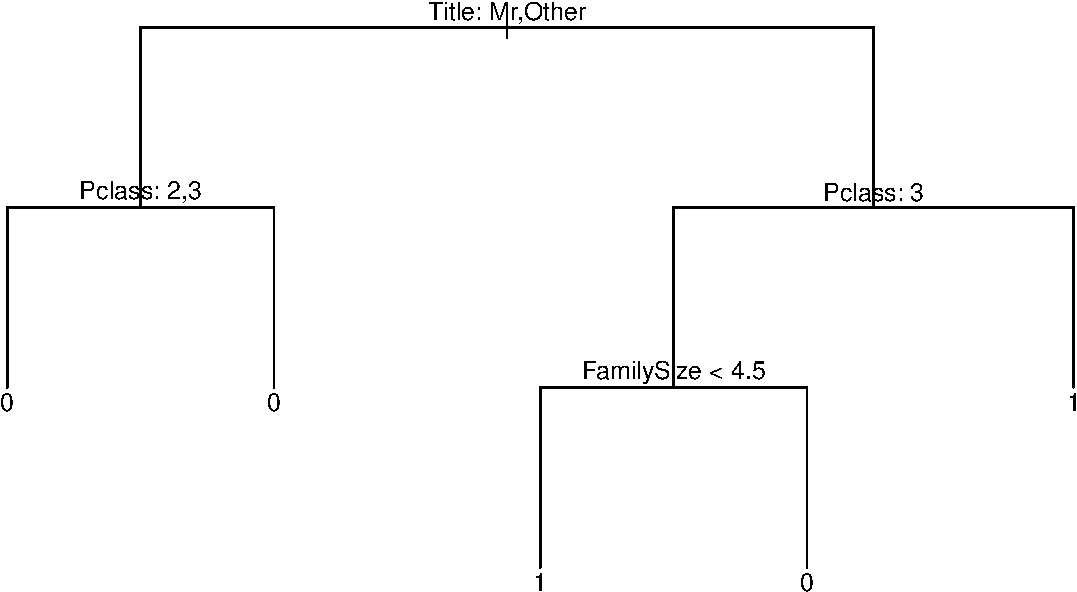
\includegraphics[scale=0.58]{tree-entropy-tree}

	\end{frame}

	\begin{frame}{Pacchetto \textit{tree} con Entropia - Pruning}
		\lstinputlisting[firstline=249, lastline=258]{../titanic-decision-trees.R}
		
		\vfill
		
		\begin{columns}
			\column{0.5\textwidth}
			\centering
			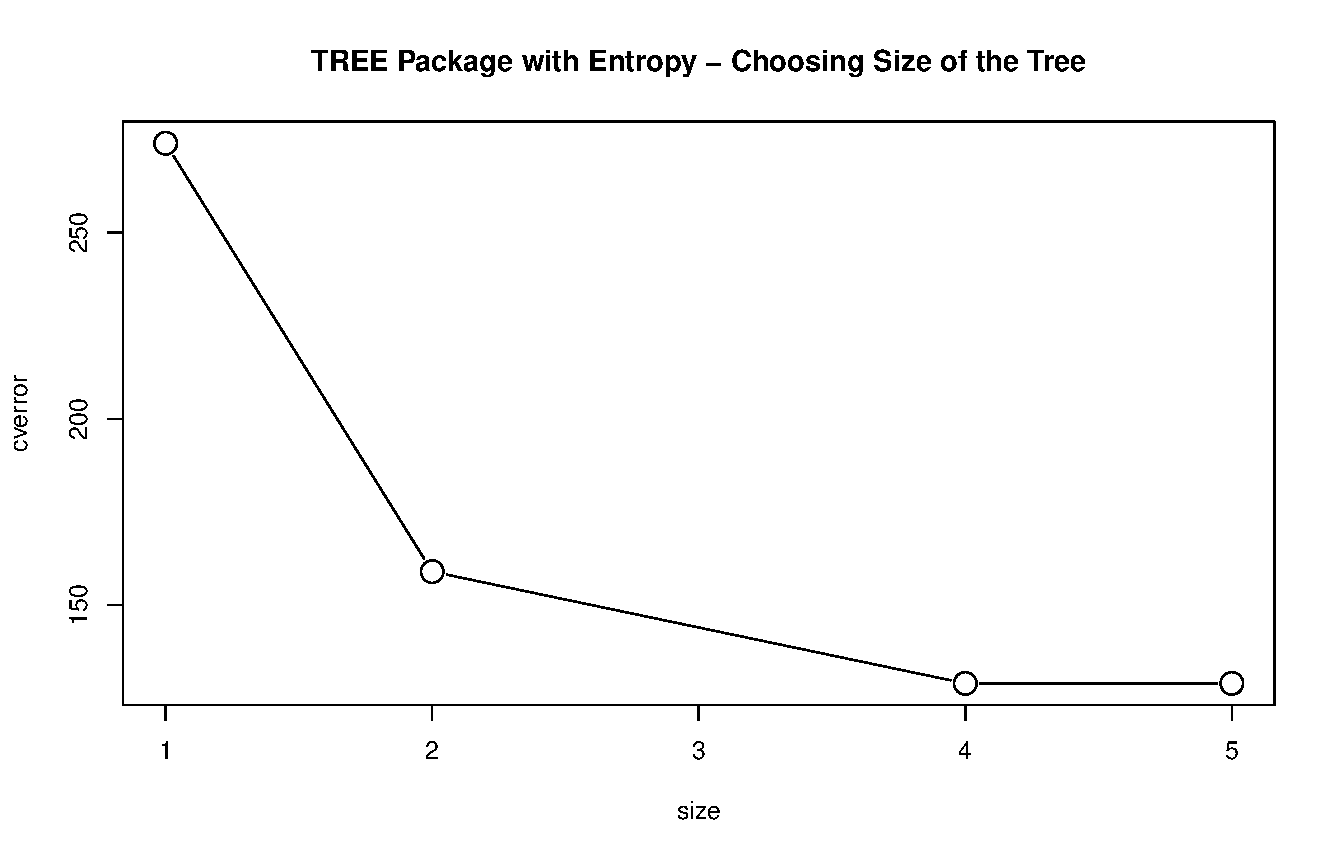
\includegraphics[scale=0.26]{tree-entropy-size-plot}
			\column{0.5\textwidth}
			\centering
			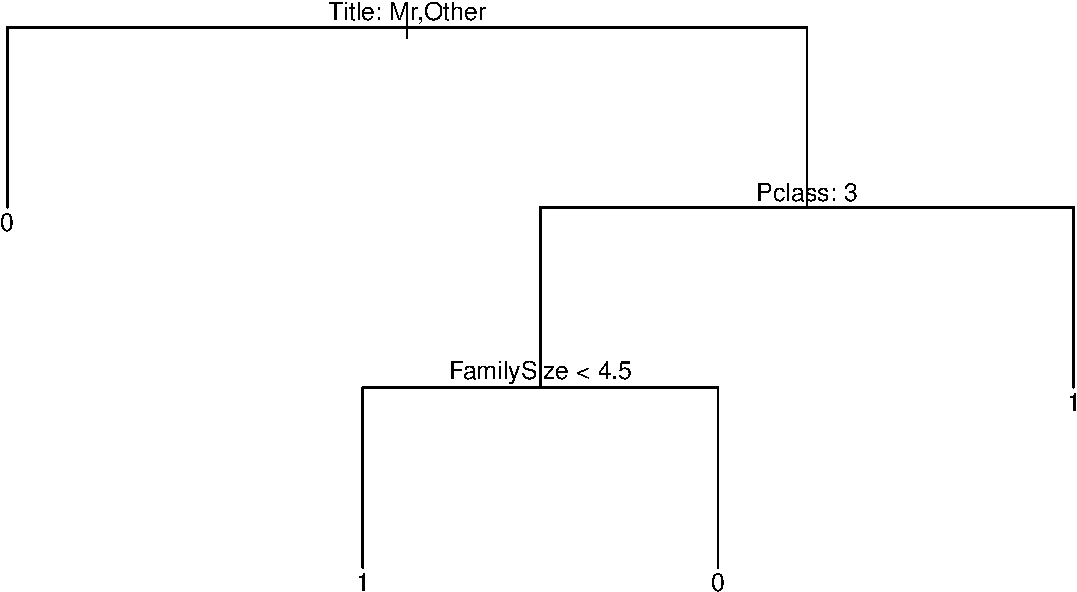
\includegraphics[scale=0.3]{tree-entropy-pruned}
		\end{columns}	
	\end{frame}

	\begin{frame}{Pacchetto \textit{tree} con Gini - Costruzione dell'Albero}
		\lstinputlisting[firstline=270, lastline=273]{../titanic-decision-trees.R}
		
		\vfill
		
		\centering
		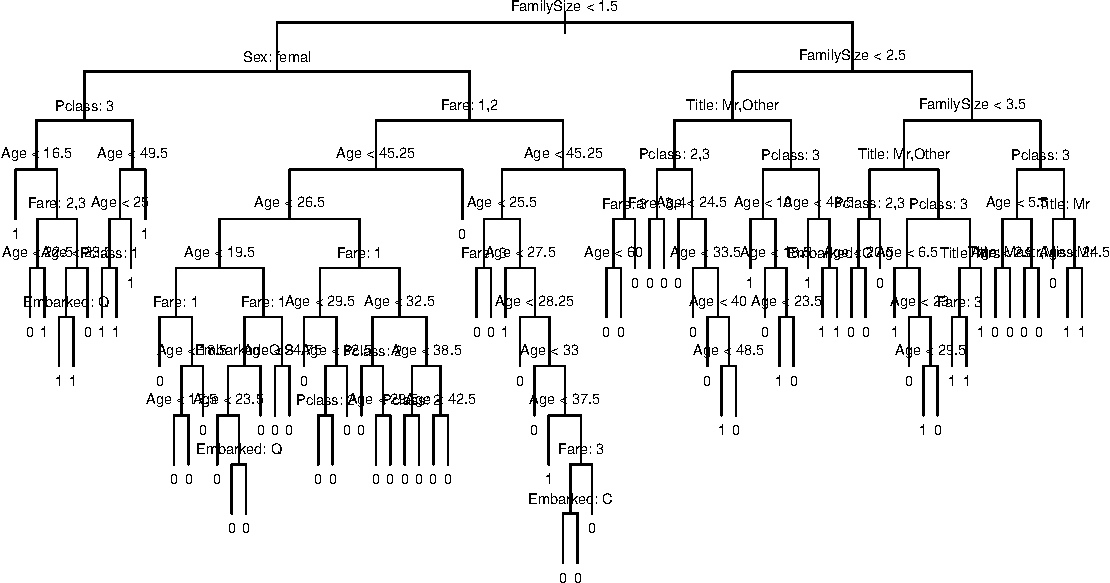
\includegraphics[scale=0.58]{tree-gini-tree}
		
	\end{frame}
	
	\begin{frame}{Pacchetto \textit{tree} con Gini - Pruning}
		\lstinputlisting[firstline=282, lastline=291]{../titanic-decision-trees.R}
		
		\begin{columns}
			\column{0.5\textwidth}
			\centering
			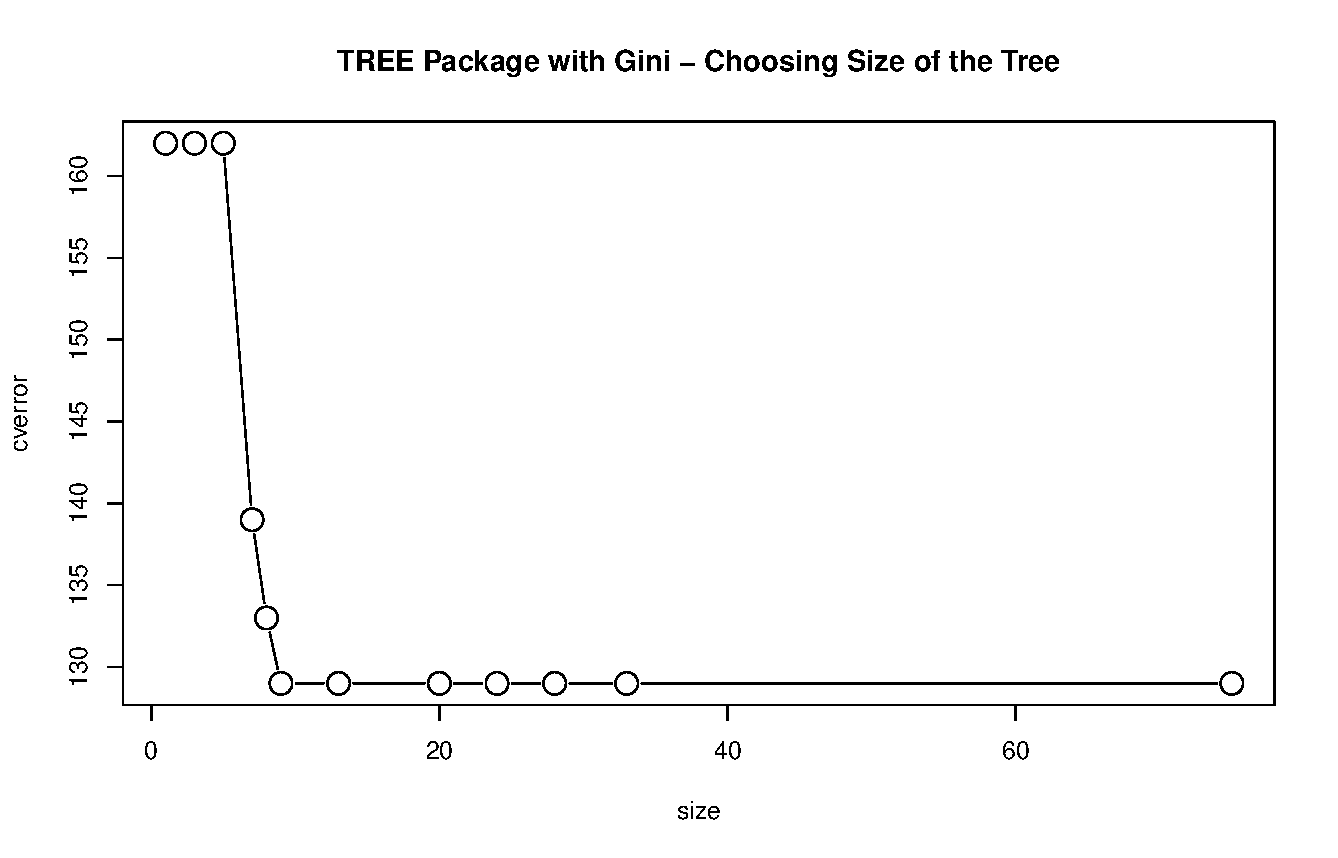
\includegraphics[scale=0.26]{tree-gini-size-plot}
			\column{0.5\textwidth}
			\centering
			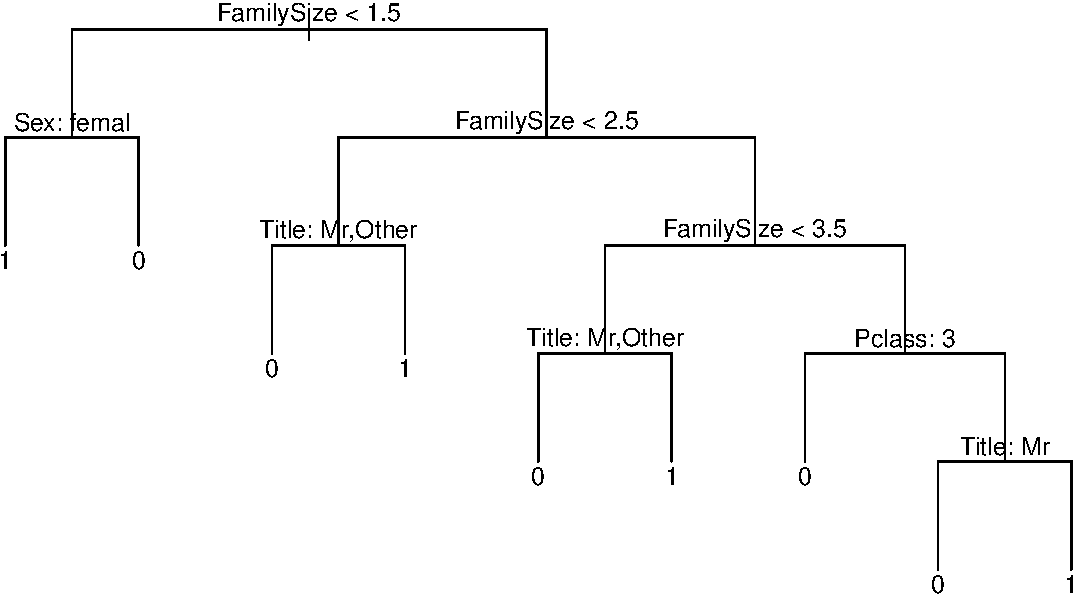
\includegraphics[scale=0.3]{tree-gini-pruned}
		\end{columns}	
	\end{frame}

	\begin{frame}{Pacchetto \textit{rpart}}		
		\begin{block}{Caratteristiche Principali}
			\begin{itemize}
				\item Reimplementazione moderna del pacchetto tree.
				\item Più efficiente, molte più parti vengono eseguite in codice C.
				\item Maggior controllo per gestire eventuali valori mancanti.
				\item Offre maggiore flessibilità durante la crescita degli alberi.
				\item Vengono offerti circa 9 parametri per la modellazione.
				\item Split di default con Gini. In	alternativa Entropia.
				\item La dimensione minima di ogni nodo deve essere 20 (default).
				\item La profondità massima dell'albero è pari a 30 (default).
				\item Algoritmo greedy, come il precedente.
			\end{itemize}
		\end{block}
	\end{frame}

	\begin{frame}{Pacchetto \textit{rpart} con Gini - Costruzione dell'Albero}
		\lstinputlisting[firstline=307, lastline=309]{../titanic-decision-trees.R}
		
		\vfill
		
		\centering
		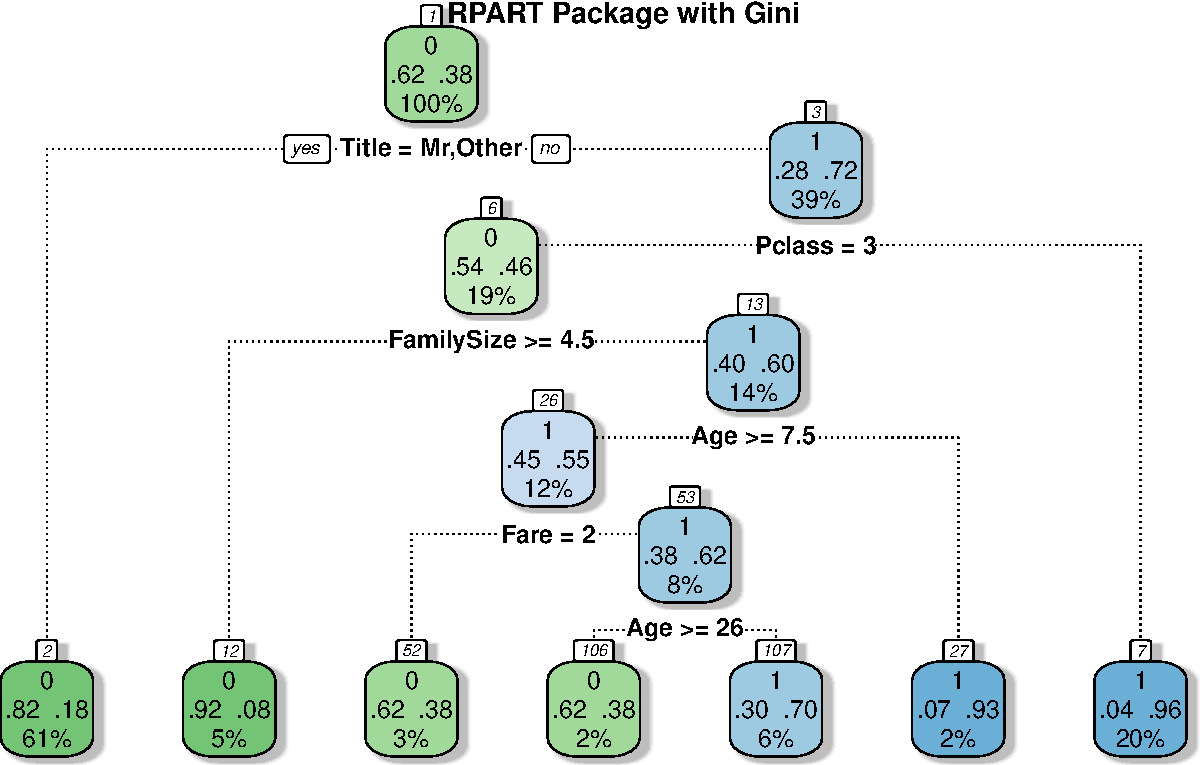
\includegraphics[scale=0.46]{rpart-gini-tree}
		
	\end{frame}

	\begin{frame}{Pacchetto \textit{rpart} con Gini - Pruning}
		\lstinputlisting[firstline=318, lastline=323]{../titanic-decision-trees.R}
		
		\vfill
		
		\begin{columns}
			\column{0.5\textwidth}
			\centering
			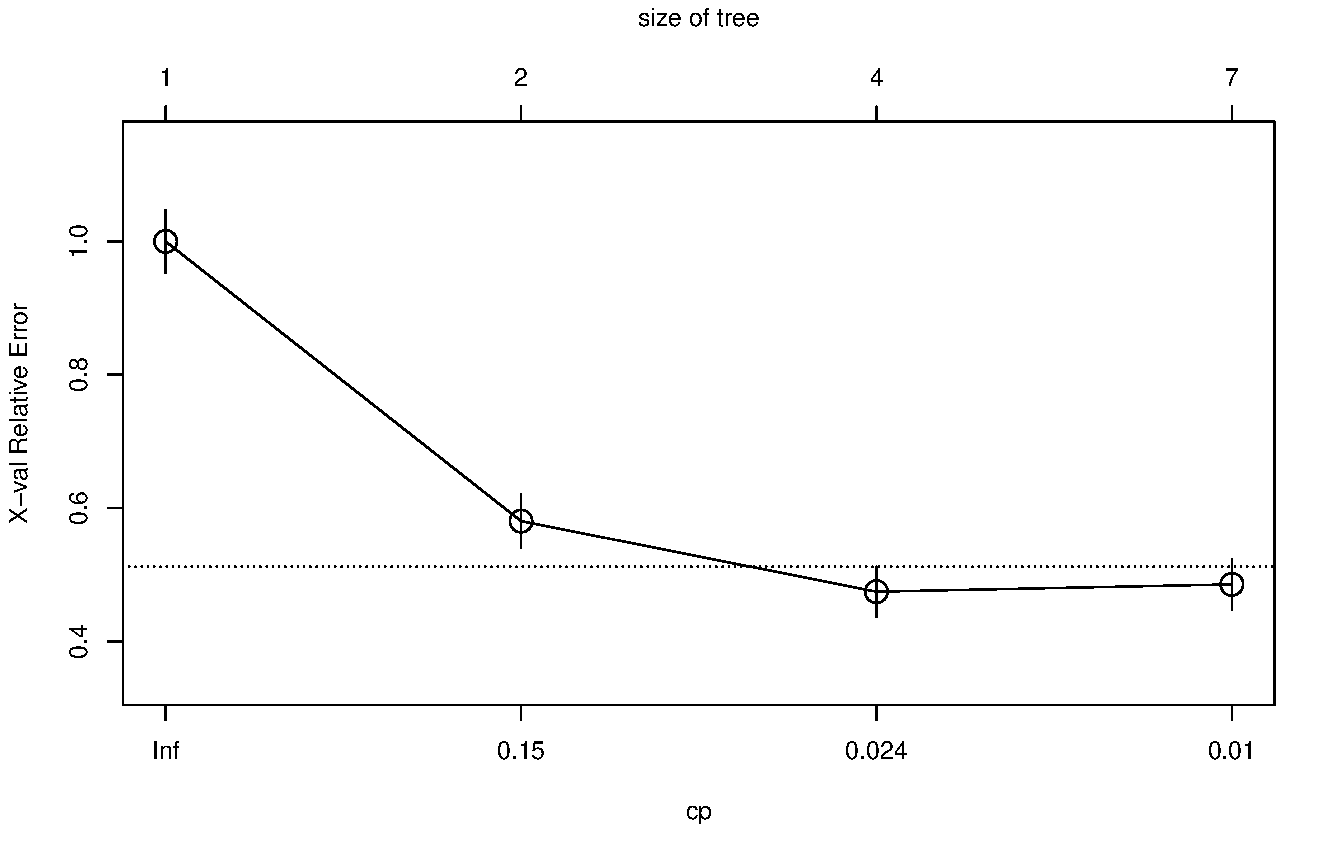
\includegraphics[scale=0.26]{rpart-gini-size-plot}
			\column{0.5\textwidth}
			\centering
			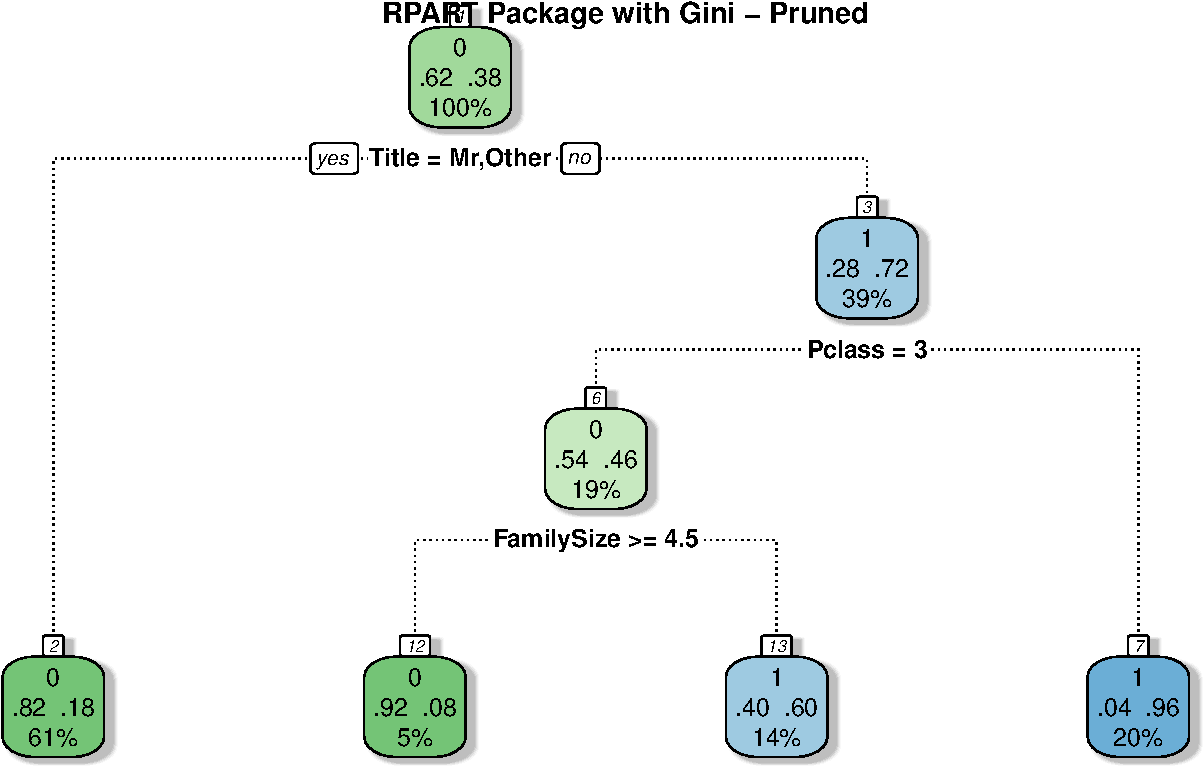
\includegraphics[scale=0.28]{rpart-gini-pruned}
		\end{columns}	
	\end{frame}

	\iffalse

	\begin{frame}{Pacchetto \textit{rpart} con Entropia - Costruzione dell'Albero}
		\lstinputlisting[firstline=335, lastline=337]{../titanic-decision-trees.R}
		
		\vfill
		
		\centering
		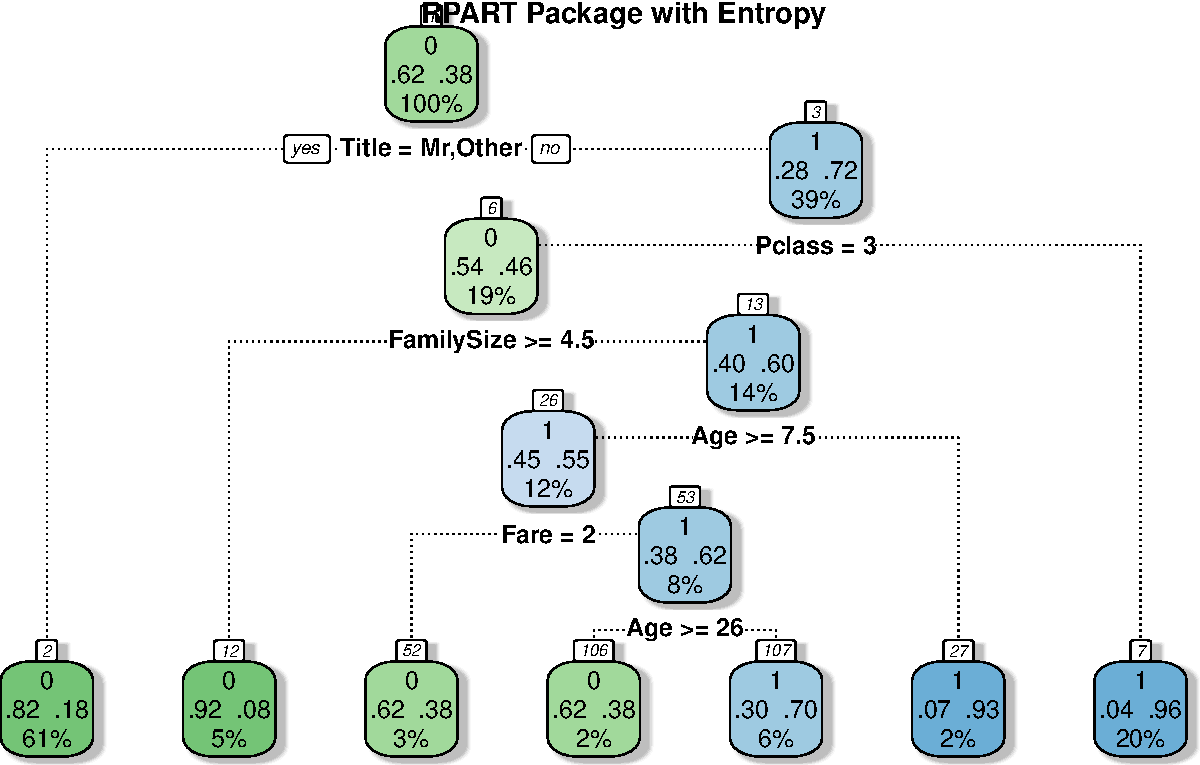
\includegraphics[scale=0.46]{rpart-entropy-tree}
		
	\end{frame}
	
	\begin{frame}{Pacchetto \textit{rpart} con Entropia - Pruning}
		\lstinputlisting[firstline=346, lastline=351]{../titanic-decision-trees.R}
		
		\vfill
		
		\begin{columns}
			\column{0.5\textwidth}
			\centering
			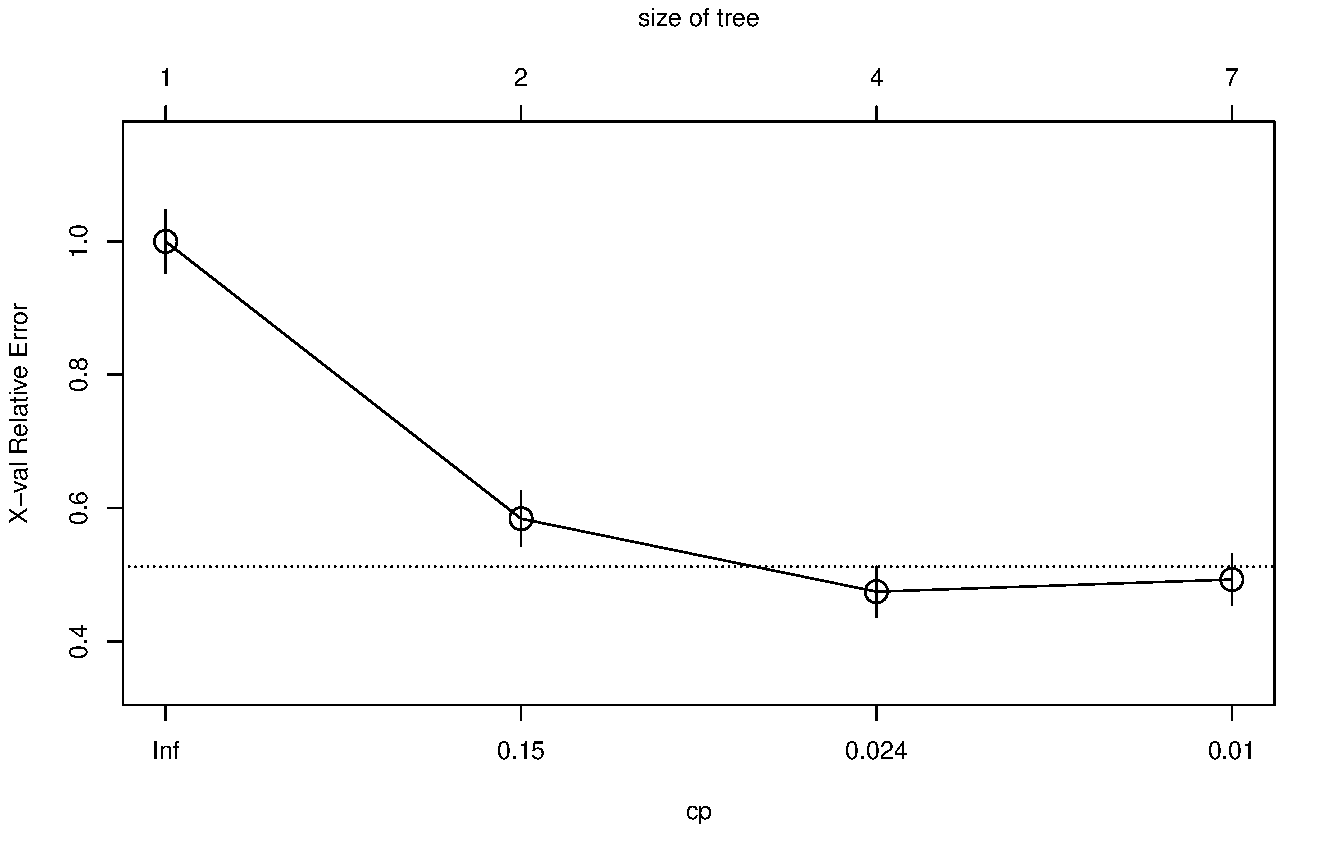
\includegraphics[scale=0.26]{rpart-entropy-size-plot}
			\column{0.5\textwidth}
			\centering
			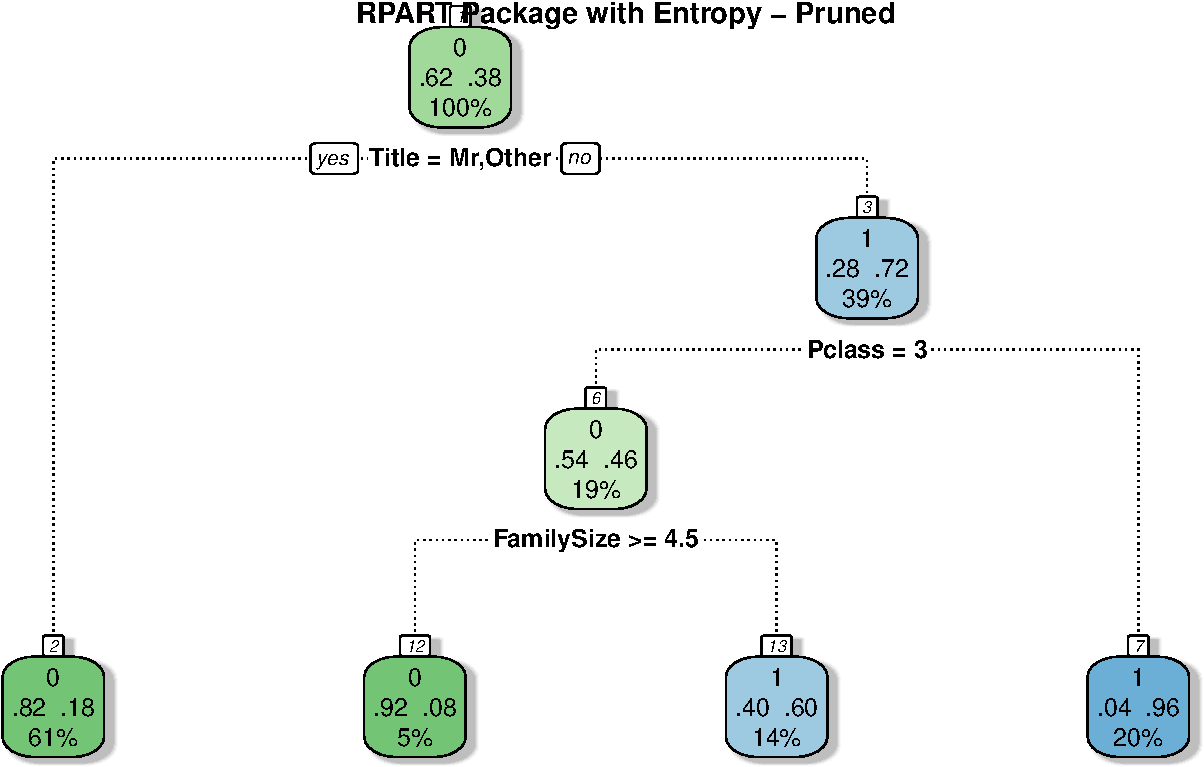
\includegraphics[scale=0.28]{rpart-entropy-pruned}
		\end{columns}	
	\end{frame}

	\fi

	\begin{frame}{Pacchetto \textit{party}}		
		\begin{block}{Algoritmo}
			\begin{enumerate}
				\item Viene effettuato un test di ipotesi nulla di indipendenza tra ogni variabile di input e la variabile risposta.
				\begin{itemize}
					\item Stop se l'ipotesi non può essere rifiutata, altrimenti seleziona la variabile con più forte associazione alla variabile di risposta.
					\item Misurata da un \textit{p-value} per test di ipotesi nulla parziale.
				\end{itemize}
				\item Split binario nella variabile di input selezionata.
				\item Ripete in modo ricorsivo i passaggi 1) e 2).
			\end{enumerate}
		\end{block}
	
		\begin{block}{Caratteristiche Principali}
			\begin{itemize}
				\item Split effettuato quando il criterio (1 - \textit{p-value}) supera il valore minimo fornito (default mincriterion = 0.95, dunque $\alpha=0.05$)
				\item Garantisce la crescita nella giusta dimensione, niente pruning.
				\item Dimensione minima di ogni nodo 20. Profondità massima $\infty$.
			\end{itemize}
		\end{block}	
	\end{frame}

	\begin{frame}{Pacchetto \textit{party} - Costruzione dell'Albero}
		\lstinputlisting[firstline=367, lastline=369]{../titanic-decision-trees.R}
		
		\vfill
		
		\centering
		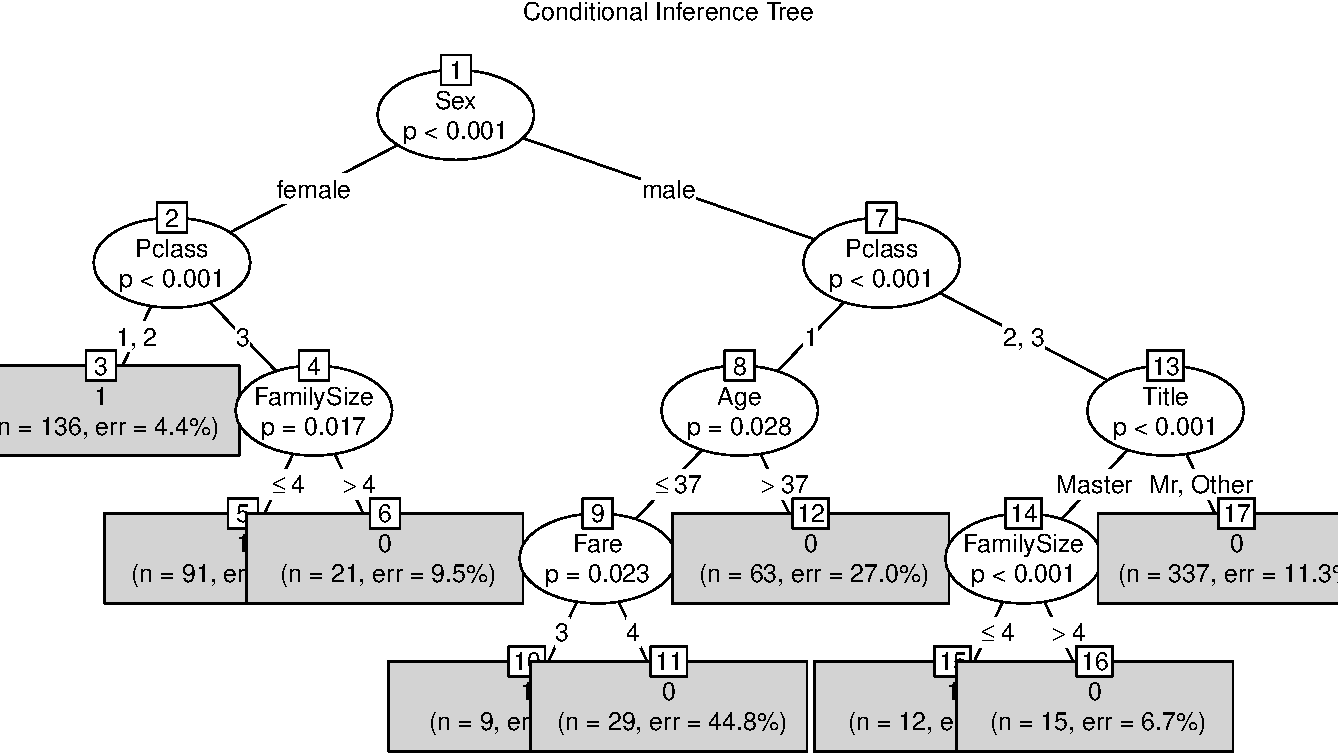
\includegraphics[scale=0.48]{party-tree}
	\end{frame}

	\begin{frame}{Pacchetto \textit{evtree}}
		\begin{block}{Caratteristiche Principali}
			\begin{itemize}
				\item Algoritmo evolutivo per l'apprendimento ottimale a livello globale di alberi di classificazione e regressione in R.
				\item Compiti intensivi completamente eseguiti in C++.
			\end{itemize}
		\end{block}
	
		\vfill
	
		\begin{algorithm}[H]
			1. Inizializzazione della popolazione.\\
			2. Valutazione di ogni individuo.\\
			\While{La condizione di terminazione non è soddisfatta}{
				a. Seleziona i genitori.\\
				b. Modifica gli individui selezionati tramite operatori di variazione.\\
				c. Valuta le nuove soluzioni.\\
				d. Seleziona i sopravvissuti per la prossima generazione.
			}
			\caption{Algoritmo \textit{evtree}}
		\end{algorithm}
	\end{frame}

	\begin{frame}{Pacchetto \textit{evtree} - Dettagli dell'Algoritmo}

		\textbf{Inizializzazione}:
		\begin{itemize}
			\item Regola di split generata casualmente in un insieme di alberi, nel \textit{root node}.
		\end{itemize}
		\textbf{Selezione del Genitore}:
		\begin{itemize}
			\item Ogni albero viene selezionato una sola volta per essere modificato.
		\end{itemize}
		\textbf{Operatori di Variazione}:
		\begin{itemize}
			\item Quattro operatori di mutazione e un operatore di crossover.
			\item In ogni fase di modifica, uno casualmente per ogni albero.
		\end{itemize}
		\textbf{Funzione di Valutazione}:
		\begin{itemize}
			\item Rappresenta i requisiti a cui la popolazione dovrebbe adattarsi. 
			\item Massimizzare la precisione e minimizzare la complessità.
		\end{itemize}
		\textbf{Selezione dei Sopravvissuti}:
		\begin{itemize}
			\item Solo la soluzione prima della modifica o quella dopo viene mantenuta. 
		\end{itemize}
		\textbf{Terminazione}:
		\begin{itemize}
			\item La qualità del 5\% dei migliori alberi si stabilizza per 100 iterazioni, ma non prima di 1000.
			\item Se non converge termina dopo un numero di iterazioni dato in input.
			\item Output: albero con la massima qualità in base alla funzione di valutazione.
		\end{itemize}	
	\end{frame}

	\begin{frame}{Pacchetto \textit{evtree} - Costruzione dell'Albero}
		\lstinputlisting[firstline=385, lastline=387]{../titanic-decision-trees.R}
		
		\vfill
		
		\centering
		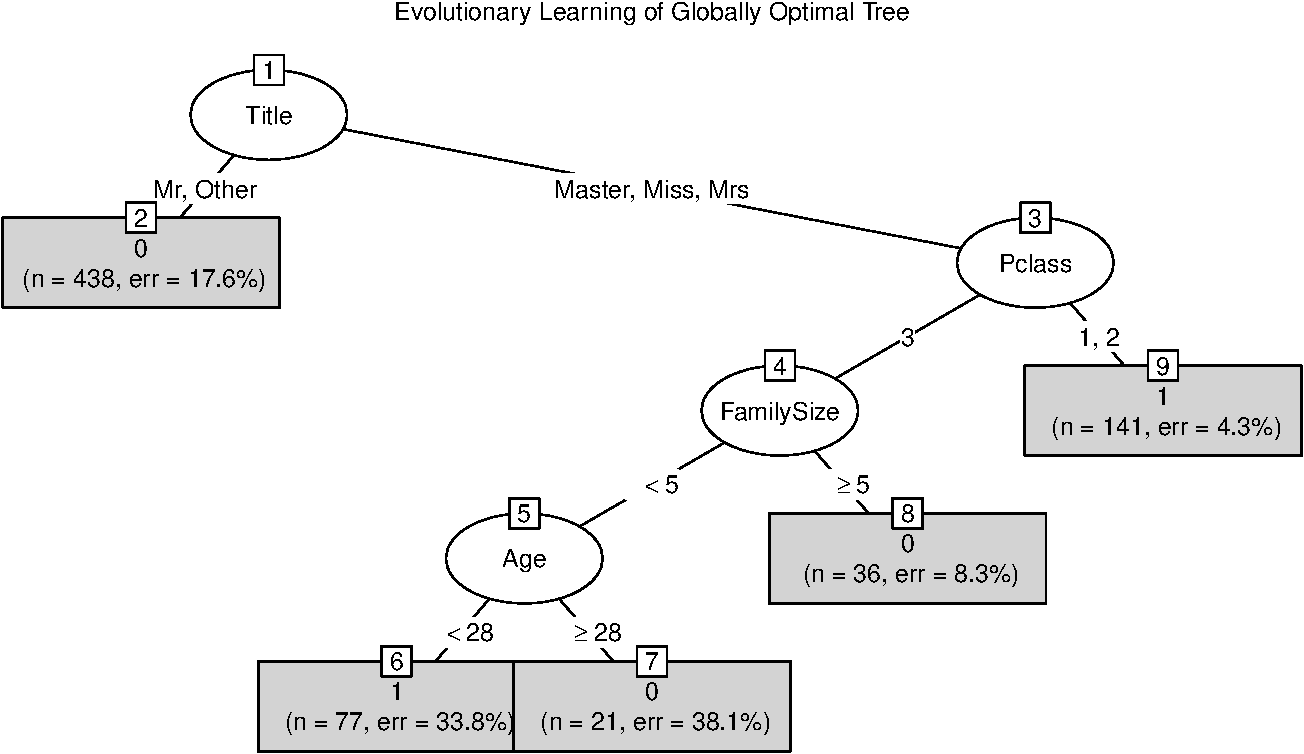
\includegraphics[scale=0.48]{evtree-tree}
	\end{frame}

	\begin{frame}{Pacchetto \textit{randomForest}}
		\begin{itemize}
			\item Il bagging riduce l'overfitting, ma non risolve completamente il problema.
			\item Un piccolo numero di predittori tende a dominare sugli altri.
			\item Selezionati nei primi split, influenzano le forme degli alberi nella foresta.
			\item Aumentano correlazioni tra gli alberi, ostacolano riduzione della varianza.
		\end{itemize}
	
		\begin{block}{Caratteristiche Principali}
			\begin{itemize}
				\item Aggira il problema usando un sottoinsieme casuale di variabili in ogni split.
				\item Evita sovrarappresentazione variabili dominanti. Foresta più diversificata.
				\item \textit{Out-of-bag} (OOB), errore di previsione medio su ciascun campione di addestramento $X_i$, utilizzando solo alberi che non hanno $X_i$ nel loro campione di bootstrap.
				\item Valuta le previsioni su quelle osservazioni che non sono state utilizzate nella costruzione del modello. Test set non necessario.
			\end{itemize}
		
			\textbf{Default:}
			
			\begin{itemize}
				\item N. di alberi (\textbf{ntree}) = 500, n. di variabili per lo split (\textbf{mtry}) = $\sqrt{n.\ predittori}$ per classificazione o \textit{mtry} = $\frac{(n.\ predittori)}{3}$ per regressione.
			\end{itemize}
		\end{block}
	\end{frame}

	\begin{frame}{Pacchetto \textit{randomForest}}
		\lstinputlisting[firstline=403, lastline=412]{../titanic-decision-trees.R}
		
		\vfill
		
		\begin{columns}
			\column{0.5\textwidth}
			\centering
			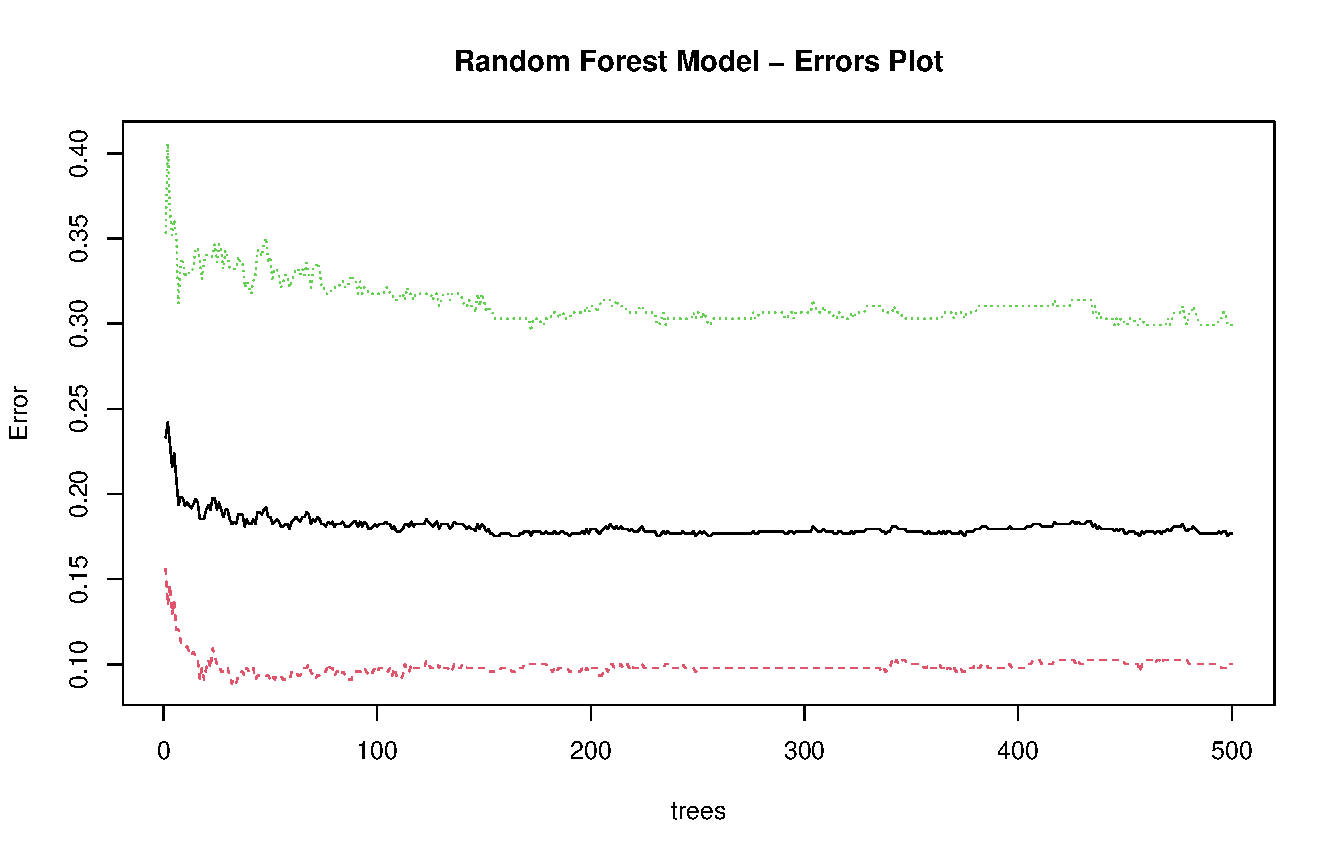
\includegraphics[scale=0.26]{randomF-errors}
			\column{0.5\textwidth}
			\centering
			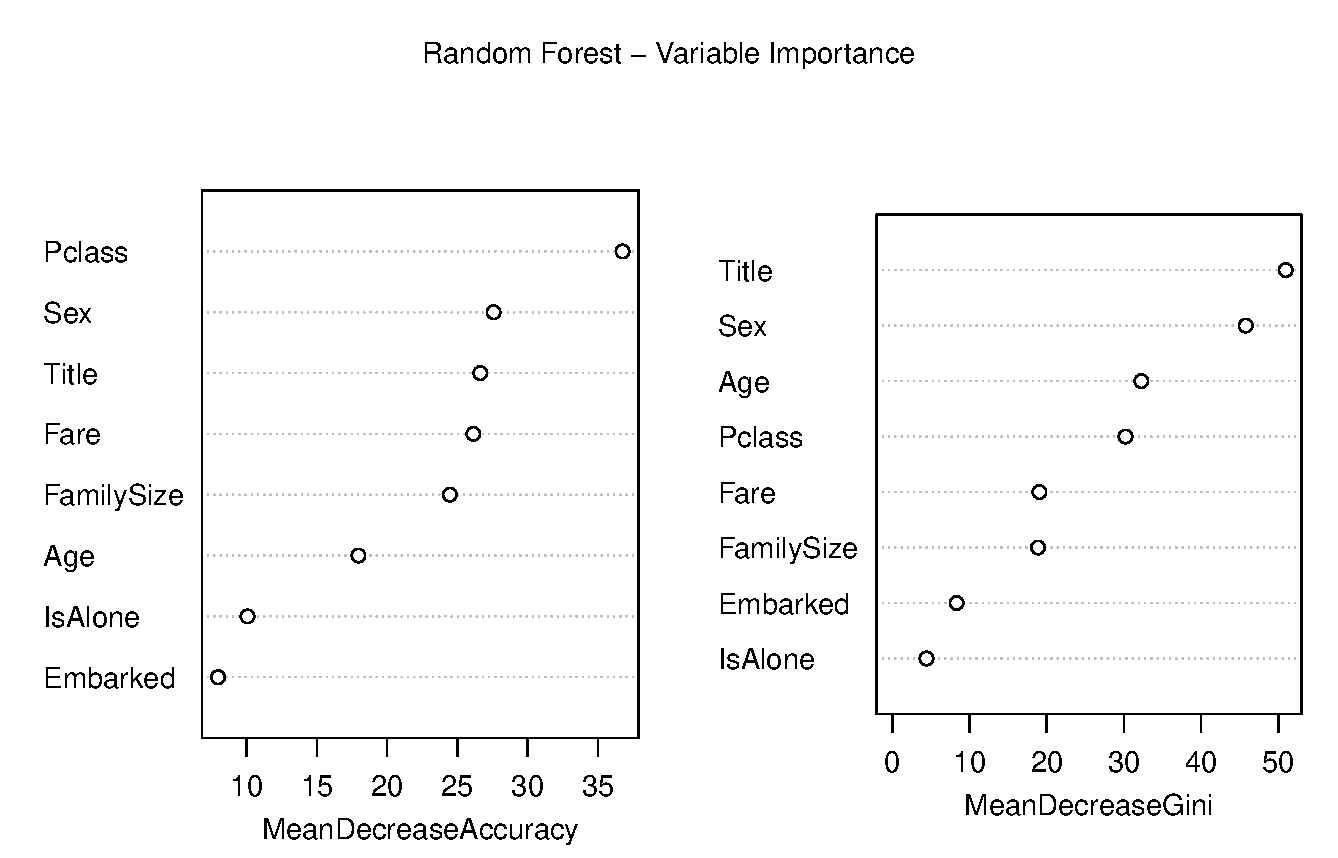
\includegraphics[scale=0.25]{randomF-var-importance}
		\end{columns}	
	\end{frame}

	\begin{frame}{Pacchetto \textit{randomForest} - Tuning dei Parametri}
		\begin{itemize}
			\item Troppi alberi possono essere eccessivi per la qualità del modello, necessità di calibrare anche il n. di variabili campionate casualmente per lo split.
			\item Cerchiamo quali sono i valori ottimali per i due parametri principali eseguendo una \textit{grid search} (\textit{ntree} tra 500 e 2000 in incrementi di 500).
		\end{itemize}
	
		\vfill
	
		\lstinputlisting[firstline=429, lastline=444]{../titanic-decision-trees.R}		
	\end{frame}

	\begin{frame}{Pacchetto \textit{randomForest} - Risultati del Tuning dei Parametri}
		\begin{columns}
			\column{0.5\textwidth}
			\centering
			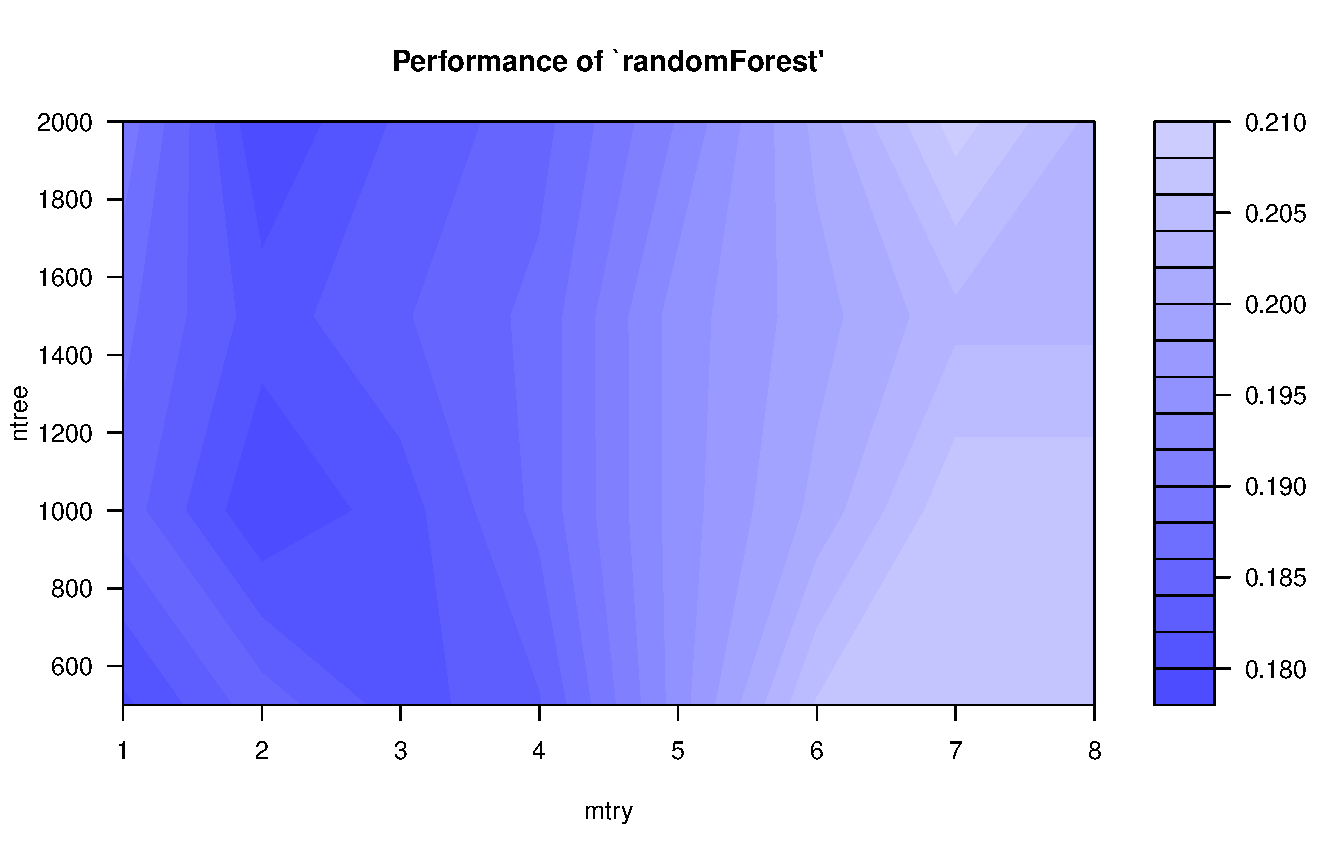
\includegraphics[scale=0.26]{randomF-tuned-performance}
			\column{0.5\textwidth}
			\centering
			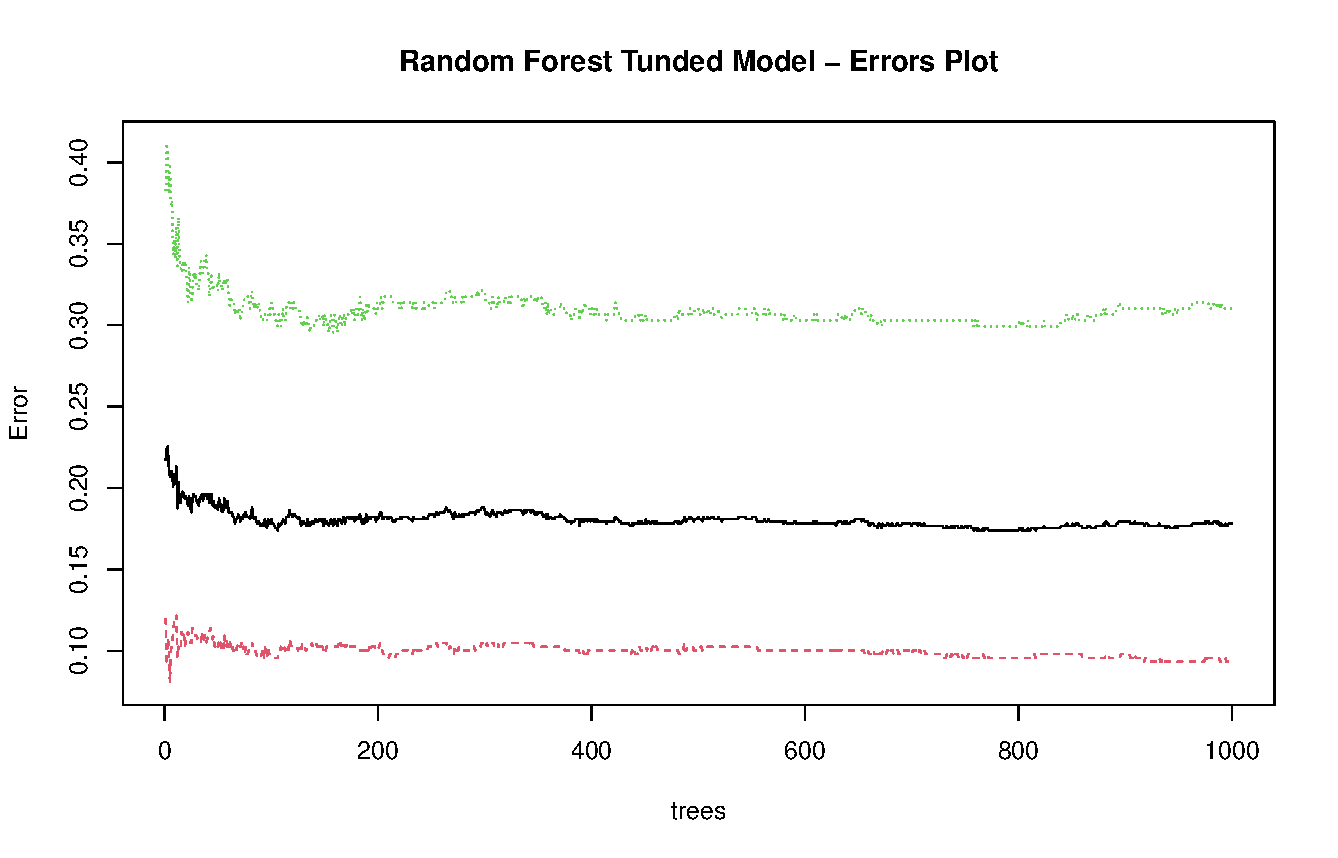
\includegraphics[scale=0.26]{randomF-tuned-errors}
		\end{columns}
		\begin{columns}
			\column{0.5\textwidth}
			\centering
			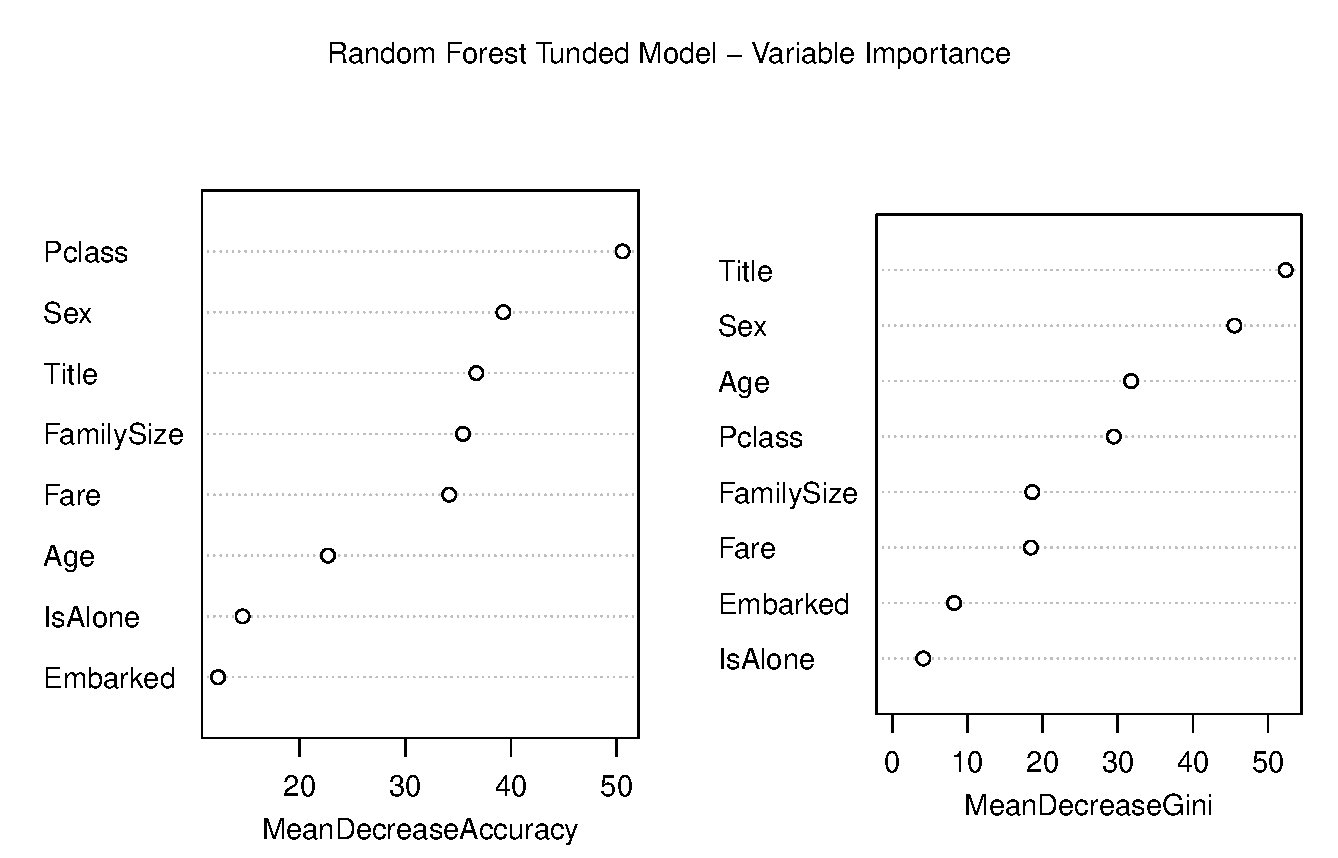
\includegraphics[scale=0.26]{randomF-tuned-var-importance}
			\column{0.5\textwidth}
			\centering
			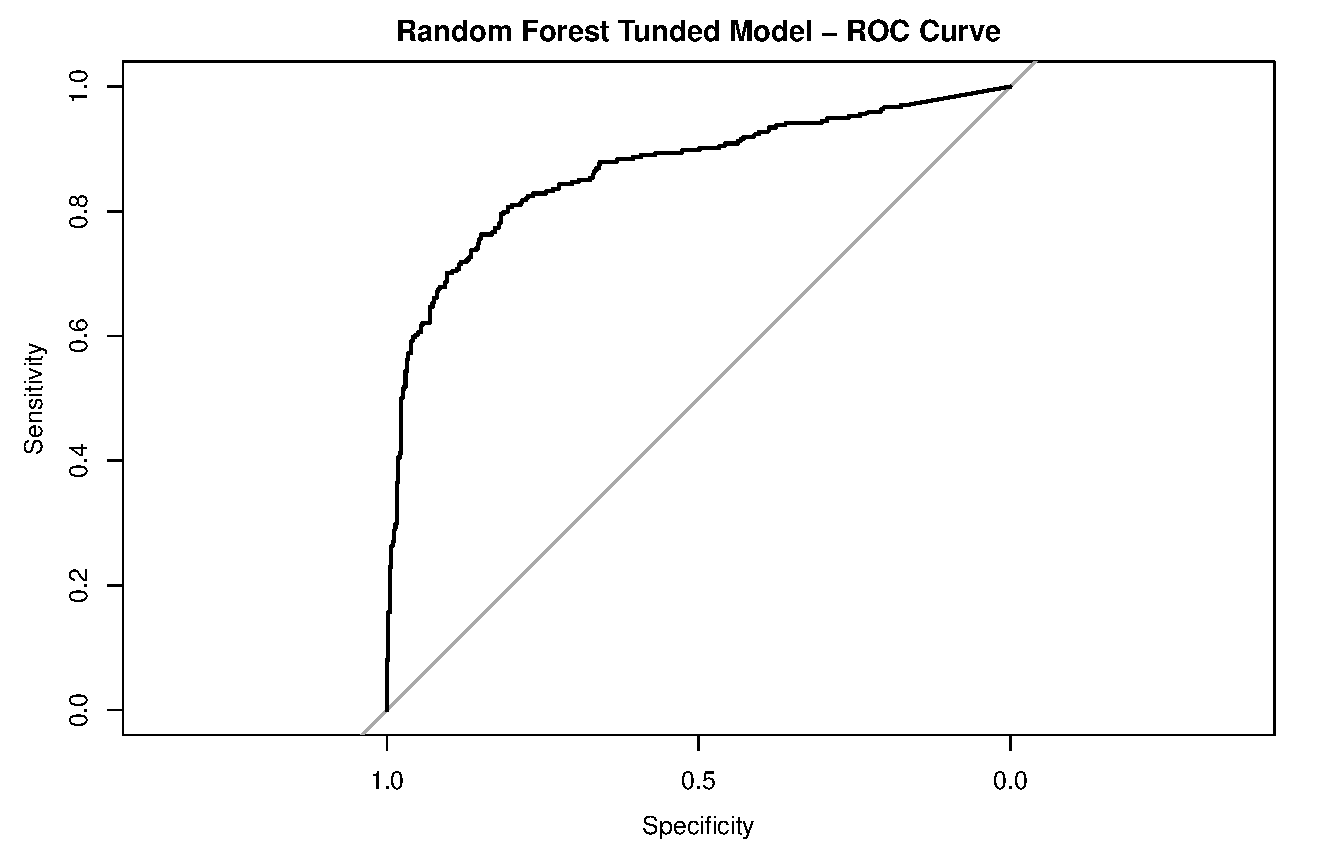
\includegraphics[scale=0.26]{randomF-tuned-roc-curve}
		\end{columns}
	\end{frame}

	\begin{frame}{Confronto tra Pacchetti - Matrici di Confusione}
		\begin{columns}
			\column{0.33\textwidth}
			\centering
			\begin{table}[]
				\resizebox{\textwidth}{!}{  
				\begin{tabular}{|c|c|c|}
					\hline
					\multicolumn{3}{|c|}{\textbf{tree - Entropia}}                                          \\ \hline
					& \textbf{Not Survived}                  & \textbf{Survived}                       \\ \hline
					\textbf{Not Survived} & \cellcolor[HTML]{32CB00}98     & \cellcolor[HTML]{CB0000}13     \\ \hline
					\textbf{Survived}     & \cellcolor[HTML]{CB0000}12     & \cellcolor[HTML]{32CB00}55     \\ \hline
					\textbf{Accuracy}     & \multicolumn{2}{c|}{\cellcolor[HTML]{FCFF2F}\textbf{85.95\%}} \\ \hline
				\end{tabular}
			}
			\end{table}
			\column{0.33\textwidth}
			\centering
			\begin{table}[]
				\resizebox{\textwidth}{!}{  
					\begin{tabular}{|c|c|c|}
						\hline
						\multicolumn{3}{|c|}{\textbf{tree - Gini}}                                          \\ \hline
						& \textbf{Not Survived}                  & \textbf{Survived}                       \\ \hline
						\textbf{Not Survived} & \cellcolor[HTML]{32CB00}99     & \cellcolor[HTML]{CB0000}19     \\ \hline
						\textbf{Survived}     & \cellcolor[HTML]{CB0000}11     & \cellcolor[HTML]{32CB00}49     \\ \hline
						\textbf{Accuracy}     & \multicolumn{2}{c|}{\cellcolor[HTML]{FCFF2F}\textbf{83.15\%}} \\ \hline
					\end{tabular}
				}
			\end{table}
			\column{0.33\textwidth}
			\centering
			\begin{table}[]
				\resizebox{\textwidth}{!}{  
					\begin{tabular}{|c|c|c|}
						\hline
						\multicolumn{3}{|c|}{\textbf{rpart - Gini}}                                          \\ \hline
						& \textbf{Not Survived}                  & \textbf{Survived}                       \\ \hline
						\textbf{Not Survived} & \cellcolor[HTML]{32CB00}98     & \cellcolor[HTML]{CB0000}13     \\ \hline
						\textbf{Survived}     & \cellcolor[HTML]{CB0000}12    & \cellcolor[HTML]{32CB00}55     \\ \hline
						\textbf{Accuracy}     & \multicolumn{2}{c|}{\cellcolor[HTML]{FCFF2F}\textbf{85.95\%}} \\ \hline
					\end{tabular}
				}
			\end{table}
		\end{columns}
		\begin{columns}
			\column{0.33\textwidth}
			\centering
			\begin{table}[]
				\resizebox{\textwidth}{!}{  
					\begin{tabular}{|c|c|c|}
						\hline
						\multicolumn{3}{|c|}{\textbf{party}}                                          \\ \hline
						& \textbf{Not Survived}                  & \textbf{Survived}                       \\ \hline
						\textbf{Not Survived} & \cellcolor[HTML]{32CB00}95     & \cellcolor[HTML]{CB0000}13     \\ \hline
						\textbf{Survived}     & \cellcolor[HTML]{CB0000}15     & \cellcolor[HTML]{32CB00}55     \\ \hline
						\textbf{Accuracy}     & \multicolumn{2}{c|}{\cellcolor[HTML]{FCFF2F}\textbf{84.27\%}} \\ \hline
					\end{tabular}
				}
			\end{table}
			\column{0.33\textwidth}
			\centering
			\begin{table}[]
				\resizebox{\textwidth}{!}{  
					\begin{tabular}{|c|c|c|}
						\hline
						\multicolumn{3}{|c|}{\textbf{evtree}}                                          \\ \hline
						& \textbf{Not Survived}                  & \textbf{Survived}                       \\ \hline
						\textbf{Not Survived} & \cellcolor[HTML]{32CB00}100     & \cellcolor[HTML]{CB0000}13     \\ \hline
						\textbf{Survived}     & \cellcolor[HTML]{CB0000}10     & \cellcolor[HTML]{32CB00}55     \\ \hline
						\textbf{Accuracy}     & \multicolumn{2}{c|}{\cellcolor[HTML]{FCFF2F}\textbf{87.08\%}} \\ \hline
					\end{tabular}
				}
			\end{table}
			\column{0.33\textwidth}
			\centering
			\begin{table}[]
				\resizebox{\textwidth}{!}{  
					\begin{tabular}{|c|c|c|}
						\hline
						\multicolumn{3}{|c|}{\textbf{randomForest}}                                          \\ \hline
						& \textbf{Not Survived}                  & \textbf{Survived}                       \\ \hline
						\textbf{Not Survived} & \cellcolor[HTML]{32CB00}98     & \cellcolor[HTML]{CB0000}14     \\ \hline
						\textbf{Survived}     & \cellcolor[HTML]{CB0000}12     & \cellcolor[HTML]{32CB00}54     \\ \hline
						\textbf{Accuracy}     & \multicolumn{2}{c|}{\cellcolor[HTML]{FCFF2F}\textbf{85.39\%}} \\ \hline
					\end{tabular}
				}
			\end{table}
		\end{columns}
	\end{frame}

	\begin{frame}
		
		\centering
		\huge \textbf{Grazie dell'Attenzione}
		
		\vfill
		
		\centering
		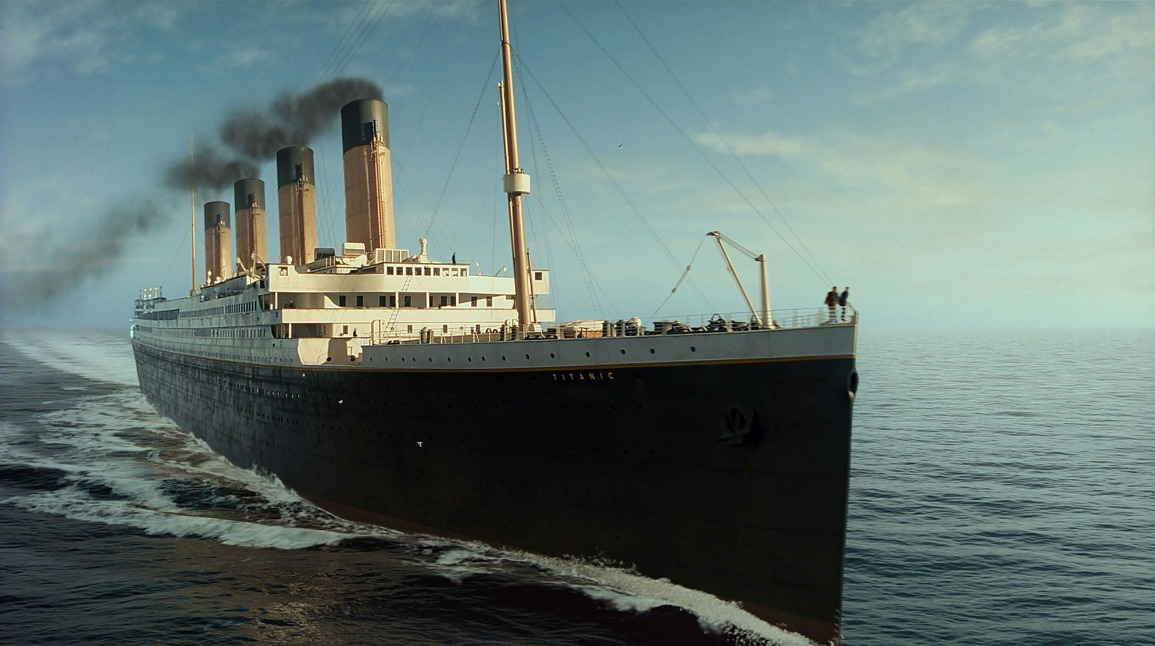
\includegraphics[scale=0.27]{titanic-sailing}
		
	\end{frame}

\end{document}